\documentclass[12pt]{article}
\usepackage{lmodern}
\usepackage[T1]{fontenc}
\usepackage[dvips,letterpaper,margin=0.75in,bottom=0.75in]{geometry}
\usepackage{cancel}
\usepackage{graphicx}
\usepackage{braket}
\usepackage{latexsym,amssymb,amsmath}
\usepackage{pdfpages}
\usepackage{xcolor}
\usepackage{capt-of}
\usepackage{amsmath}
\usepackage{cite}
\newcommand{\tcr}{\textcolor{red}}
\newcommand{\tcb}{\textcolor{blue}}


\usepackage[american,fulldiode]{circuitikz}
\tikzset{component/.style={draw,thick,circle,fill=white,minimum size =0.75cm,inner sep=0pt}}

\begin{document}
\ctikzset{bipoles/thickness=1}
\ctikzset{bipoles/length=.6cm}


%%%%%%%%%%%%%%%%%%%%%%%%%%%%%%%%%%%%%%%%%%%%%%%%%%%%%%%%%%%%%%%%
%%%%%%%%%%%%%%%%%%%%%%%%%%%%%%%%%%%%%%%%%%%%%%%%%%%%%%%%%%%%%%%%
\title{Proposal for Revising the Undergraduate Curriculum \\
Department of Physics and Astronomy}
%%%%%%%%%%%%%%%%%%%%%%%%%%%%%%%%%%%%%%%%%%%%%%%%%%%%%%%%%%%%%%%%
%%%%%%%%%%%%%%%%%%%%%%%%%%%%%%%%%%%%%%%%%%%%%%%%%%%%%%%%%%%%%%%%

\maketitle

\section{History and Status of the Proposal}

This proposal has been developed over the past three years within the
Department of Physics and Astronomy, 
led by the undergraduate curriculum committee.
The proposal was subjected to an extensive vetting process that
involved assigned department readers who were not involved in
formulating the initial plan.  The proposal was unamimously supported
by the department in a December 2021 vote.
All new courses, modified courses, and
discontinued courses are already under review in the 
UC Davis Integrated Curriculum Management System (ICMS).


The impact of the proposal outside of the Department of Physics 
and Astronomy is
expected to be minimal. The proposal leaves PHY 7 and 9 unchanged,
apart from a long overdue clean up of the mathematics prerequisites,
which make them consistent with the equivalencies accepted by the
Department of Mathematics, and increases the options available to
students.  The proposal does eliminate PHY 9HE, but a search of the
current course catalog does not indicate any majors that explicitly
list PHY 9HE as a requirement (even an alternate) or prerequisite.

Our revisions to the computational curriculum
involves the replacement of
PHY 102 and PHY 104B with
PHY 45, 110L, 112L, and 115L.
The third quarter of electricity and magnetism, PHY 110C is also 
eliminated, with the mathematical review that used to
be part of the sequence taken up in PHY 9 and PHY 104.
Details concerning how these affect each specific major in the 
program are found in the corresponding sections 4-6.
(A third quarter of quantum physics, PHY 115C, will eventually be added
as an elective, partly
in recognition of the rapid development and growth of quantum
information science,
but this change is several years in the future and hence not currently
in ICMS.)

PHY 116ABC will evolve into PHY 117,118.
None of these will affect majors outside of physics,
nor will they necessitate any additional instructors.
See Appendix A1 for a complete list of course content changes.

\section{Objectives of the Proposal}


The changes proposed here reflect three main observations: \\
\tcb{\bf [i.\,\,\,\,]}  Workload over four years of study was imbalanced, with too few physics
courses in the sophomore year, and too many in the junior year. \\
\tcb{\bf [ii.\,\,]}  
%% Transfer enrollment has risen dramatically and integration
%% of transfer students with four year students, who have somewhat
%% different backgrounds, needed to be improved. \\
Integration between transfer students and
four-year students, who have somewhat different backgrounds, needed to be
improved. Our recent departmental Climate Survey confirmed this by showing a
huge satisfaction gap between the groups. \\
\tcb{\bf [iii.]}  The curriculum did not reflect the explosive growth
in computational methods and their applications.

This document is organized as follows:  In the remainder of this
Section 2 we review the
current schedules for four-year majors and transfer students.  We
identify the deficiencies in some detail.  In Sections 3--6 we discuss
the proposed Physics BS, Astrophysics, Applied Physics, and Physics AB 
requirements, providing Tables with specific
course listings and timings, and catalog content changes.
Appendix A summarizes course content changes (A1); 
contains discussion of the implications of
this proposal on the different branches of physics-- theoretical (A2), 
computational (A3), and experimental(A4); 
and, finally, the prerequisite structure (A5) of
the program.
Appendix B contains example course syllabi.
Appendix C contains details of implementation.


An example schedule of student coursework without the revisions
proposed here is shown in Table~\ref{tbl:current-honors} for students
taking honors physics.  An example schedule for students that transfer
to UC Davis for their junior year is shown in
Table~\ref{tbl:current-transfers}.  There are many different
trajectories through our program, but most are some variation on these
two.  For consistent comparisons, all the example schedules for BS
Physics majors in this proposal assume the students take 122A and one
capstone course in the winter, and two capstone courses in the spring.
Many other lab courses and offerings are possible.

\captionof{table}{\label{tbl:current-honors} An example schedule
  satisfying the {\em current requirements} for an undergraduate
  physics major that takes the 9H series and 122A. Physics course
  numbers are shown with the number of units in parenthesis.  Math
  courses start with M.  Courses in italics are electives or have at
  least two different offerings per year. Course CAP is a capstone
  elective, and course X is any advanced elective.}
\begin{center}
\begin{tabular}{|l|l|l|l|}
\hline
Year      & Fall    & Winter & Spring \\
\hline
Freshman  & 9HA(5)     & 9HB(5)     & 9HC(5) \\
          & {\it M21B(4)}  & {\it M21C(4)}  & {\it M21D(4)} \\
\hline
Sophomore & 9HD(5)     & 9HE(5)     & 40(3)     \\
          & {\it M22A(3)}     & {\it M22B(3)} & {\it 80(4)} \\
\hline
Junior    & 104A(4) & 105B(4) & 110B(4)\\
          & 105A(4) & 110A(4) & 115A(4)\\
          & 102(1)  &    &     \\
\hline
Senior    & 110C(4) & {\it 122A(4)} & {\it X(3-4)}\\
          & 112(4)  & {\it CAP(4)}   & {\it X(3-4)}\\
          & 115B(4) & {\it CAP(4)}   & {\it CAP(4)}\\

\hline 
\end{tabular}
\end{center}

\captionof{table}{\label{tbl:current-transfers} An example schedule
  satisfying the {\em current requirements} for an undergraduate
  physics major that transfers to UC Davis in their junior year and
  takes 122A.  Most of our incoming transfer students have not taken
  an equivalent course for at least one of PHY 9D, 40, or 80.  This
  example considers the extreme case where they have completed none of
  these courses upon arrival in the junior year.  Physics course
  numbers are shown with the number of units in parenthesis.  Courses
  in italics are electives or have at least two different offerings
  per year.  Course CAP is a capstone elective, and course X is any
  advanced elective.}

\begin{center}
\begin{tabular}{|l|l|l|l|}
\hline
Year      & Fall    & Winter & Spring \\
\hline
Junior    & 9D(4)   & 105B(4) & 40(3)   \\
          & 104A(4) & 110A(4) & 110B(4) \\
          & 105A(4) & {\it 80(4)}   & 115A(4) \\
          & 102(1)  &         & \\
\hline
Senior    & 110C(4) & {\it 122A(4)} & {\it X(3-4)}\\
          & 112(4)  & {\it CAP(4)}   & {\it X(3-4)}\\
          & 115B(4) & {\it CAP(4)}   & {\it CAP(4)}\\
\hline 
\end{tabular}
\end{center}

There are some deficiencies in the current course of study:
\begin{itemize}

\item Physics majors who complete 9HD or 9D in the fall of their
  sophomore year have little to do for the rest of the year.  The
  honors sequence has 9HE, but that course does not contain any
  content which is a prerequisite for upper division class work.  The
  recent addition of 40 and 80 is helpful in that it provides
  something for students to do during this time, but the problem still
  remains that they do not make progress on the upper division core
  coursework, and 80 is not taken by all students.  The result of
  this stalling is that the junior and senior years are a race to
  complete the degree requirements, leaving very little flexibility or
  time for advanced electives.

\item Students that transfer to UC Davis for their junior year face a
  wall of coursework that they have to handle in the first quarter:
  math methods, mechanics, and modern physics.  Many also take 102,
  which instructors have found challenging to teach within the
  workload limits of a one-unit course.  For many students, these are
  also the first courses they encounter that require solving
  challenging homework problems.  We have two trains of students
  running through our program and the fall of their junior year is the
  train wreck where they collide.

\item The current curriculum does not include sufficient computing
  practice for our students.  It is useful to consider what a physics
  degree would look like if we taught calculus the same way we teach
  computing.  Students would arrive their freshman year and take an
  introductory calculus course.  Then, they would take their physics
  courses, which would never mention calculus.  At some point in their
  junior or senior year, they would take a one quarter course called
  ``Calculus in Physics'' which would attempt to show all the ways we
  use calculus in physics.  Our students are experts at calculus
  because they learn how to use the tool, and then apply it, again and
  again, throughout their coursework.  To remain relevant in the
  modern world (or even the world from 20 years ago) our majors need
  more practice in the use of computing as an essential tool for
  solving physics problems.

\item Four-year students typically graduate with around 180 units.
  Within the College of Letters and Science, we are allowed to require
  a maximum of 110 units in our majors.  The current BS physics major
  requires a minimum of 108 units to complete.  Fitting the canon of
  undergraduate physics into such a tight space is extremely
  challenging.  Students complain that we waste time teaching some
  topics again and again (e.g. Special Relativity from scratch) while
  completely dropping other topics (e.g. Classical Hamiltonians).  The
  problem is particularly acute for applied physics majors, where core
  material must be dropped to make space for coursework outside of
  physics.

\item The prerequisite structure of the upper division courses creates
  many tiers.  As an extreme example, 122 requires 112, which requires
  115A, which requires 104A and 105A, both of which require the 9
  series.  This, combined with the rapid pace, leaves very little
  flexibility for students once they start their junior year.  For
  example, missing any of the four-unit courses in the junior year of
  Table~\ref{tbl:current-honors} requires an exception to
  prerequisites or an extra year to graduate.
\end{itemize}

This proposal aims to make significant improvements on these
issues, focused on the following considerations:

\vskip0.10in \noindent \tcb{$\bullet$}
Use the sophomore pause more productively, lower the junior year brick wall.
\vskip0.04in \noindent \tcb{$\bullet$}
Provide more practice and training in computational physics
\vskip0.04in \noindent \tcb{$\bullet$}
Our niche: designing, programming, and validating numerical models and algorithms.
\vskip0.04in \noindent \tcb{$\bullet$}
Computing and analytic skills are complementary, it's not one vs the other.
\vskip0.04in \noindent \tcb{$\bullet$}
Avoid reteaching and missed topics.
\vskip0.04in \noindent \tcb{$\bullet$}
Simplify prerequisite structure and reliably deliver prerequisite material.
\vskip0.04in \noindent \tcb{$\bullet$}
We must preserve a two year graduation path for students that transfer in their junior year.
\vskip0.04in \noindent \tcb{$\bullet$}
We cannot exceed 110 units of required coursework (including math).


\newpage


\section{Proposed BS Requirements}

The proposed required courses for a BS in physics are presented in
Tables~\ref{tbl:prep} and \ref{tbl:depth}.  The math prerequisites for
lower division coursework are broken out separately in
Table~\ref{tbl:math-prereqs}.  Example schedules are presented in
Tables~\ref{tbl:proposed-honors}-\ref{tbl:proposed-transfers}.

A primary feature of this proposal is that incoming transfer students
now overlap in some courses with sophomores who took the honors
physics sequence.  This eliminates the stalling of our four-year
students while relieving some of the intense academic pressure on
incoming transfer students.  Our experience has been that the best of
our transfer students perform as well as the best of our four-year
students, once they have sufficient time to adjust, and this proposal
gives them that time.  Accelerating students who took the honors
sequence also provides tremendous additional flexibility to their
schedule.  The example schedule in Table~\ref{tbl:proposed-honors}
assumes the student takes each class nearly as soon as possible,
leaving ample time in their senior year for additional electives.

Transfer students who wish to complete their degree in two years are
still highly constrained, but instead of facing three upper division
courses immediately upon arrival they now start with one upper
division course.  Take the time to compare fall quarter of the junior
year in Tables~\ref{tbl:current-transfers} and
\ref{tbl:proposed-transfers}; this is a major feature of this
proposal.  This gentle introduction does not come at the cost of
dramatically increased unit loads later on: transfer students can
still complete the degree without exceeding 13 units of physics
coursework in any quarter.

The college imposes a limit of 110 units of required coursework,
including prerequisites, for any major.  Within a particular major,
options that exceed this limit are permitted, as long as a path that
stays below the limit is available.  The current BS physics major
requires a minimum of 108 units.  This proposal takes advantage of the
remaining two units and brings the minimum to 110 units.  This
slightly increases total unit pressure on students, which particularly
affects those transfer students who have only two-years to absorb
them.  However, the proposal replaces the one-unit course PHY 102 with
the more appropriately sized four-unit PHY 45 course.  Also, the major
stress point for transfer students is in their first quarter, which
this proposal substantially improves.  The proposal also adds
significantly more schedule flexibility, which should also help
alleviate pressure.

\newpage
\vskip 2cm
\captionof{table}{\label{tbl:prep}Preparatory Subject Matter}
\vskip 0.25cm
\noindent
Units:  52-54. *: recommended.\\
See Table~\ref{tbl:math-prereqs} for math prerequisites.\\
\begin{tabular}{|llllll|}
\hline
Course & & Units & Offered & Prereqs & Name \\
\hline
MAT & 21A & 4 & FWS & & Differential Calculus\\ 
    & 21B & 4 & FWS &  & Integral Calculus \\ 
    & 21C & 4 & FWS &  & Partial Derivatives and Series\\ 
    & 21D & 4 & FWS &  & Vector Analysis\\
\hline
    & one of:  & & & & \\
MAT & 22A & 3 & FWS &  & Linear Algebra\\
    & 27A & 3 & FWS &  & Linear Algebra\\
    & 67  & 4 & FWS &  & Mod. Linear Algebra\\
\hline
MAT & 22B & 3 & FWS &  & Differential Equations\\
    & or  & & & & \\
MAT & 27B & 3 & FWS &  & Differential Equations\\ 
\hline
\hline

PHY & 9A & 5 & FS &  & Class. Physics {\it (Class. Mech.)}\\
& 9B & 5 & FW & 9A/9HA    & Class. Physics {\it (Waves, Thermo, Optics)}\\
    & 9C & 5 & WS & 9B  & Class. Physics {\it (Elec. and Magn.)}\\ 
    & 9D & 4 & FS & 9C & Mod. Physics {\it (Rel. and QM)}\\ 
\hline
&or&&\\
\hline
PHY & 9HA & 5 & F &  & Honors Physics {\it (Class. Mech.)}\\ 
    & 9HB & 5 & W & 9A/9HA  & Honors Physics {\it (Rel. and Stat. Mech.)}\\ 
    & 9HC & 5 & S & 9HB  & Honors Physics {\it (Waves and QM)}\\ 
    & 9HD & 5 & F & 9HC   & Honors Physics {\it (Elec. and Magn.)}\\ 
\hline
\hline
PHY & 40  & 3 & F & & Introduction to Physics Computation \\ 
    & 45  & 4 & W & 40,9C/9HD & Computational Physics\\ 
    & 80  & 4 & FS & 9C/9HD,40        & Experimental Techniques \\
    & 185* & 1 & S & & Careers in Physics \\ 
    & 190* & 1 & F & & Careers in Physics \\ 
\hline
\end{tabular}\\

\newpage
\vskip 2cm
\captionof{table}{\label{tbl:depth}Depth Subject Matter}
\vskip 0.5cm
\noindent
Units:  39-43. *: recommended, $\parallel$: concurrently.\\
\begin{tabular}{|llllll|}
\hline
Course & & Units & Offered & Prereqs & Name \\
\hline

PHY & 104A & 4 & FS & 9C/9HD,MAT 22B   & Mathematical Physics \\ 
    & 105A & 4 & W & 9C/9HD, & Classical Mechanics I\\
    &      &   &   & MAT 22A, $\parallel$22B & \\
    & 105B & 4 & S & 105A,40$\dagger$          & Classical Mechanics II\\ 
    & 110A & 4 & W & 104A,9C/9HD             & Electricity and Magnetism I\\
    & 110B & 4 & S & 110A                     & Electricity and Magnetism II\\
    & 110L & 1 & S & 45/ECS 36B, $\parallel$110B & Comp. Lab in Electricity and Magn. \\
    & 112  & 4 & F & 104A,9D/9HD      & Thermo. and Stat. Mech.\\    
    & 112L & 1 & F & 45/ECS 36B, $\parallel$112/CHE 110A  & Comp. Lab in Statistical Mechanics \\ 
    & 115A & 4 & F & 104A,105A,9D/9HD & Quantum Mechanics I \\
    & 115B & 4 & W & 115A             & Quantum Mechanics II \\
    & 115L & 1 & W & 115A/CHE 110C,$\parallel$115B*  & Comp. Lab in Quantum Mechanics \\
           & & & & 45/ECS 36B & \\
    & 115C* & 4 & S & 115B,45/ECS 36B& Appl. of Quantum Mechanics\\ 
\hline
\hline
PHY & 117 & 4 &  F & 80              & Phys. Instr. with A\&D Electronics.  \\
    & 118 & 4 &  W & 80,45/ECS 36B   & Phys. Instr. for Data Acquisition. \\ 
\hline
    & or & & & & \\
\hline
PHY & 122A/B & 4 & WS & 80,104A,105A,110B & Advanced Physics Laboratory \\  
    &  & & & \& $\parallel$112 $\parallel$115A&  \\  
\hline
\end{tabular}\\ 
\noindent
$\dagger$:  Instructor permission may be obtained to take PHY 105B without the PHY 40 prerequisite.
\noindent
{\bf Electives:} Additional electives to bring the total number of 3
or more unit upper division courses to 14, including at least three
from capstone courses.  (4-5 courses, totaling 15-20 units with
current offerings) Includes at most one from PHY 194H series, 195, 198, or 199
and excludes PHY 160.
\noindent
{\bf Total Units:} 110-113

\newpage
\vskip 2cm \captionof{table}{ Math prerequisite for lower division
  courses related to this proposal.  Where indicated, course grades
  are the minimum accepted to meet prerequisites.  The prerequisites
  for the math courses are set by the math department and are only
  reported here.  Where possible, math prerequisites for physics
  courses adopt the same choices made by the math department with
  respect to equivalent math coursework.}
\label{tbl:math-prereqs}
\begin{center}
\begin{tabular}{|llll|}
\hline
Course & & Math Prereqs (Minimum Grade)& Name \\
\hline
MAT & 16A & & Short Calc.\\
    & 16B & 21A/21AH/17A/16A(C-) & Short Calc.\\
    & 16C & 21B/21BH/17B/16B(C-) & Short Calc.\\
    & 17A &                      & Calc (Bio\&Med)\\
    & 17B & 21A/21AH/17A/16A(C-) & Calc (Bio\&Med)\\
    & 17C & 17B(C-)              & Calc (Bio\&Med)\\
    & 21A &                      & Calculus \\
    & 21B & 21B/21BH(C-) or 17A(B) & Calculus \\
    & 21C & 21B/21BH/17C/16C(C-) or 17B(B) & Calculus\\
    & 21D & 21C/21CH(C-) or 17C(B) & Calculus \\
    & 22A & 21C/21CH/17C/16C(C-)    & Linear Algebra \\
    & 22B & 67/22A(C-)           & Diff. Eqs. \\
    & 67  & 21C/21CH(C-)           & Mod. Lin. Alg. \\
\hline
\hline
PHY & 9A & 21B/21BH/17C/16C(C-) or 17B(B) & Class. Physics\\
    & 9B & 21C/21CH(C-) or 17C(B) & Class. Physics\\
    & 9C & 21D(C-) & Class. Physics\\
    & 9D & 22A(C-) or 67(C-) & Class. Physics\\
    &    & $\parallel$22B & \\
\hline
\hline
PHY & 9HA & $\parallel$21B/$\parallel$21BH & Hon. Physics\\
    & 9HB    & 21B/21BH(C-) & Hon. Physics \\
    & 9HC    & 21C/21CH & Hon. Physics \\
    & 9HD    & 21D  & Hon. Physics \\
\hline
PHY & 45     & $\parallel$22B & Computational Physics \\
\hline
\end{tabular}
\end{center}


\newpage
\captionof{table}{ An example schedule satisfying the
  {\em proposed requirements} for an undergraduate physics major that
  takes the 9H series and 122A. Physics course numbers are shown with
  the number of units in parenthesis.  Math courses start with M.
  Courses in italics are electives or have at least two different
  offerings per year. Course CAP is a capstone elective, and course X
  is any advanced elective.  Rate is 3-9 physics units per quarter in
  junior and senior year.}
\label{tbl:proposed-honors}
\begin{center}
\begin{tabular}{|l|l|l|l|}
\hline
Year      & Fall    & Winter & Spring \\
\hline
Freshman  & 9HA(5)       & 9HB(5)        & 9HC(5) \\
          & {\it M21B(4)} & {\it M21C(4)}  & {\it M21D(4)}\\
\hline
Sophomore & 9HD(5)       & 105A(4)      & 105B(4) \\
          & {\it M22A(3)} & {\it M22B(3)} & {\it 104A(4)} \\
          & 40(3)        & 45(4)       & {\it 80(4)}  \\
\hline
Junior    & 115A(4) & 115B+L(5)  & {\it 115C(4)}\\
          & 112+L(5)  & 110A(4)  & 110B+L(5)\\
\hline
Senior    & {\it X(3-4)} & {\it 122A(4)} & {\it CAP(4)} \\
          &              & {\it CAP(4)} & {\it CAP(4)} \\
\hline  
\end{tabular}
\end{center}


\vskip 2cm
\captionof{table}{ An example schedule satisfying the
  {\em proposed requirements} for an undergraduate physics major that
  takes the 9 series and 122A. Physics course numbers are shown with
  the number of units in parenthesis.  Math courses start with M.
  Courses in italics are electives or have at least two different
  offerings per year. Course CAP is a capstone elective, and course X
  is any advanced elective.  Rate is 7-13 physics units per quarter in
  junior and senior year.}
\label{tbl:proposed-nonhonors}
\begin{center}
\begin{tabular}{|l|l|l|l|}
\hline
Year      & Fall    & Winter & Spring \\
\hline
Freshman  & {\it M21A(4)}  & {\it M21B(4)}  & {\it M21C(4)}\\
          &               &               & {\it 9A(5)} \\
\hline
Sophomore & {\it M21D(4)}  & {\it M22A(3)}  & {\it M22B(3)}\\ 
          & {\it 9B(5)}    & {\it 9C(5)}    & {\it 9D(4)} \\
          & 40(3)          &                & {\it 80(4)} \\
\hline
Junior   & {\it 104A(4)}   & 105A(4)       & 105B(4) \\
         & {\it X(3-4)}      & 110A(4)       & 110B+L(5) \\         
         &                 & 45(4)         & \\

\hline
Senior   & 115A(4)    & 115B+L(5)     & {\it 115C(4)} \\
         & 112+L(5)   & {\it 122A(4)} & {\it CAP(4)} \\
         &            & {\it CAP(4)}   & {\it CAP(4)}  \\
\hline 
\end{tabular}
\end{center}

\newpage
\captionof{table}{An example schedule satisfying the
  {\em proposed requirements} for an undergraduate physics major that
  transfers to UC Davis in their junior year, without Physics 9D or 40
  equivalents, and takes 122A. Physics course numbers are shown with
  the number of units in parenthesis.  Courses in italics are
  electives or have at least two different offerings per year. Course
  CAP is a capstone elective, and course X is any advanced elective.
  Rate is 12-13 units per quarter.  Note that only one upper division
  course is required in the first quarter of junior year, compared to
  three upper division courses in the current program.  }
\label{tbl:proposed-transfers}
\begin{center}
\begin{tabular}{|l|l|l|l|}
\hline
Year      & Fall    & Winter & Spring \\
\hline
Junior   & 9D(4)         & 105A(4)   & 105B(4) \\
         & 40(3)         & 110A(4)   & 110B+L(5) \\         
         & {\it 104A(4)} & 45(4)     & {\it 80(4)} \\
\hline
Senior   & 115A(4)    & 115B+L(5)      & {\it 115C(4)} \\
         & 112+L(5)   & {\it 122A(4)} & {\it CAP(4)} \\
         & {\it X(3-4)} & {\it CAP(4)}   & {\it CAP(4)}  \\
\hline 
\end{tabular}
\end{center}

\vskip 2cm
Several new courses have been added, some are no longer offered, and
others require changes to their content:
\begin{itemize}

\item 9A-D and 9HA-D are unchanged, but their prerequisites have been
  adjusted for consistency with the math prerequisites (including
  minimum grades) used by the math department and to match existing
  policy (e.g. 9A is acceptable prerequisite for 9HB.)

\item 9HE is no longer offered.  This course is effectively an
  elective, with content that varies from instructor to instructor.
  By removing it, we allow the students in the honors sequence to
  start toward the core material sooner, leaving more time for
  advanced electives. With the more relaxed schedule in their senior
  year, it seems highly plausible that physics majors will take more
  advanced electives.

\item 104A: This course will now be offered in both fall and spring,
  as discussed further in the discussion of prerequisites.  Most
  students taking honors physics will take the course in the spring,
  while most transfer students will take the course in the fall.  Two
  offerings will remove a major bottleneck, result in smaller class
  sizes.  Most four-year students from honors physics will take the
  spring offering, whereas most incoming junior year transfer students
  will take the fall offering.  This will allow the course to be
  pitched slightly differently in each quarter, to better reflect
  student preparation.

\item 105: The timing of the 105AB sequence is adjusted to start in
  winter.  The content of 105AB should be at a level appropriate for a
  sophomore completing 9HD in the previous quarter.  There is no prerequisite for
  104A, but typically students will take 104A either concurrently with
  105B or before 105A.

\item 110: The present curriculum devotes three quarters of required
  upper division coursework to Electricity and Magnetism (110ABC).
  This proposal eliminates 110C and increases the pace of 110AB.
  Students must reliably enter 110 having adequate preparation in
  vector calculus, curvilinear coordinates, Lorentz transformation,
  relativistic mechanics, and introductory electricity and magnetism.
  This material must be covered adequately in the 9 series and 104A.

\item 112: The 115A prerequisite for 112 has been removed, and the
  treatment must rely on quantum from the PHY 9 series instead.  Fermi
  and Bose statistics will be introduced independently in 112.  PHY 9
  and 9H must consistently cover discrete energy levels from the
  particle in a box and simple harmonic oscillator.  The annual
  faculty curriculum discussion is the mechanism for ensuring this is
  so.
    
\item The 115AB sequence is extended to include an elective third
  quarter: 115C.  The prerequisites are 104A and 105A.  The elective
  third quarter, 115C, adds 45 as a prerequisite, and the course
  includes extensive computational problems.  The extra time should
  also allow coverage of new elective topics (for example Quantum
  Information Theory).  As this is an elective course, there is no
  need to implement it immediately, and it can be developed first as a
  PHY 150 course.

\item The computational courses are described in
  Section~\ref{sec:computing}. PHY 40 is updated, PHY 102 and 104B are
  dropped, and new courses PHY 45, 110L, 112L and 115L are added.

\item The traditional lab courses are discussed in
  Section~\ref{sec:labs}. PHY 80, 116A, 116B, and 116C are replaced with
  PHY 80, 117, and 118.  PHY 122A/B is unchanged.
  
\end{itemize}
Example syllabi for all courses impacted by this proposal are
presented in Section~\ref{sec:syllabi}.

This proposal is approximately neutral with respect to the cost of
instruction if we assume that the cost of electives is held constant
(we of course have no obligation to do so.)  Instructors teaching a
one-unit computation lab course will receive credit for one third of a
standard podium course.  The three new computational lab courses
together add one new instructor.  The second offering of 104A and the
new required course 45 add two new instructors.  But dropping courses
9HE, 102, 104B, 110C and replacing 116ABC with 117 and 118 frees 4.3
instructors, for a net decrease of 1.3 instructors.  If the need for
more sections of 80 requires an additional instructor (currently
typically two, although three were initially planned for 2020-2021)
there would be a decrease of 0.3 instructors.  Additional fall
offerings for 122A/B could be added as well, if needed to meet demand.

\section{Theoretical Physics}
\label{sec:theory}

At the core of any undergraduate physics degree are the following
topics in theoretical physics:
\begin{itemize}
\item Classical Mechanics (105AB): the fundamental principles of physical laws
  (e.g. least action and symmetries) are taught in a familiar and
  intuitive context. 
\item Electromagnetism (110AB): a remarkable special case of classical
  phenomena that anticipate non-Newtonian physics (e.g. special
  relativity, gauge theories).  No other force in nature can be understood so
  completely in such a straightforward fashion.  
\item Quantum Mechanics (115AB): the rules governing the microscopic world are
  different from those governing our familiar macroscopic world.  The
  rules are not intuitive but they can be codified and used to make
  quantitative predictions which can be experimentally verified.
\item Statistical Mechanics (112): the crucial statistical explanation for how
  microscopic laws ultimately produce the macroscopic world which we inhabit.
\end{itemize}

The physics department has recently adopted a procedure for
maintaining example syllabi for core courses, through an annual
faculty meeting discussion and vote.  This is the mechanism for
ensuring that prerequisite material is being appropriately and
consistently covered in the proper courses.  The example syllabi, as
presented during the first annual faculty curriculum discussion are
presented in Section~\ref{sec:syllabi}.  This proposal need not
resolve all of the issues brought up in these discussions, as these
discussions will continue, with an update and faculty vote as needed.

The major topics from the first curriculum discussion were:
\begin{itemize}
 \item It was agreed that 105A needs to cover Hamiltonian mechanics, by
   adding supplementary material to the preferred textbook (Morin).
 \item The treatment of radiation in 110AB is limited.
 \item There is support for covering waveguides in either 110AB, 80, or even 110L.   
 \item PHY 104A plays a central role in providing students with the
   analytic techniques needed for upper division coursework.  This
   course has been far too topical for the central role it plays in
   our program, and the example syllabi should be closely followed by
   future instructors.
 \item The 115AB content is presented as either the historical
   progression or spin first.  The instructors will coordinate each
   year and agree on an approach.  Sufficient review is included in
   both versions PHY 115B so that students who took 115A under a
   different progression do not miss any crucial material, such as
   particle-in-a-box, simple-harmonic oscillator, or angular momentum.

   
\end{itemize}

\section{Computational Physics}
\label{sec:computing}

One of the major objectives of this proposal is to better integrate
computational physics throughout the curriculum.  To do so, students
must master a consistent set of tools that can be relied upon in later
courses.  The course descriptions in the course catalog will not
reference specific tools, to allow this to evolve over time, but in a
consistent manner.  In this proposal, the supported computational
tools are:
\begin{itemize}
\item Scientific computing tools for Python: NumPy, SciPy, MatPlotLib,
  and Jupyter Notebooks via Anaconda
\item C/C++
\item Computer Algebra:  Mathematica or SymPy
\end{itemize}
The entire Scientific Python ecosystem is easily accessible to
students for any major OS for free through Anaconda.  No graphical
features of C/C++ will be explored.  If necessary, C++ programs will
pass data by text file to SciPy for plotting.  SymPy is not as mature
as Mathematica, but comes with the significant advantages of being
freely available within Anaconda and interoperable with SciPy.

In 2018, we added a new required course, PHY 40, which introduces
programming with both C++ and python.  This format leaves no time for
symbolic computation and little time for exploring additional features
of Scientific Python beyond the basic Python language.  In 2021, the
course was taught exclusively with Scientific Python, which was found
to be much more workable.  However, even with this reduced scope, most
students taking the course are not yet ready to do extensive
unsupervised computational work, and only manage to make significant
progress during lab sections with TA support.  For this reason, recent
instructors agree that a three unit course, with essentially no
homework, is a more appropriate format for PHY 40.

In the current program, the additional computational physics
requirement is either PHY 102 (1 unit) or 104B (4 units).  This
proposal replaces these options with a single new required four-unit
computational physics course, PHY 45.  In addition, BS physics majors
are required to take three one-unit computational lab courses:
110L,112L, and 115L.  PHY 80 is a traditional lab course, as described in
Section~\ref{sec:labs}, but it is included in this discussion as it
also includes significant computational aspect.

\begin{figure}
\begin{center}
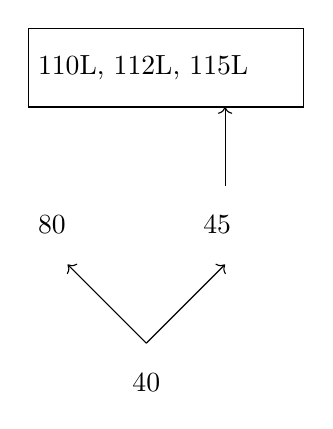
\begin{tikzpicture}
% 1st tier:
\node[right] at (1.2,0.5) {40};
%\draw (0,0) coordinate(X) -- ++(0,1) -- ++(1.8,0) |- (X);
\draw[->] (1.5,1) --(0.5,2);
\draw[->] (1.5,1) --(2.5,2);
% 2nd tier:
\node[right] at (0,2.5) {80};
%\draw (0,2) coordinate(X) -- ++(0,1.0) -- ++(1.2,0) |- (X);
\node[right] at (2.1,2.5) {45};
\draw[->] (2.5,3) --(2.5,4);
% 3rd tier:
\draw (0,4.0) coordinate(X) -- ++(0,1) -- ++(3.5,0) |- (X);
\node[right] at (0,4.5) {110L, 112L, 115L};
\end{tikzpicture}
\caption{\label{fig:comps} Prerequisite structure of computational courses.}
\end{center}
\end{figure}

The computational physics content of the required courses in this
proposal include:
\begin{itemize}
\item 40: This three-unit course has no prerequisites and assumes no
  prior knowledge of programing.  It provides an introduction to
  programming using examples from computational physics.  It includes
  a short introduction to symbolic manipulations using a computer
  algebra system.  The specific tools covered (which will not be
  included in the course description) are Scientific Python and either
  SymPy or Mathematica.

\item 45: This new four-unit course, Computational Physics, will have
  the PHY 9 series through E\&M as a prerequisite (9C/9HD) as well as
  PHY 40.  The focus will be on solving physics problems at the
  conceptual level of the 9 series using computational physics.  It
  will introduce the C++ programming language and continue using
  Scientific Python.
  
\item 80: This traditional lab course includes extensive use of
  scientific python for data analysis and presentation, including
  curve fitting and plotting scientific data.
  
\item 110L, 112L, and 115L: These three new one-unit computational lab
  courses are designed to be taken concurrently with 110B, 112, and
  115B. They are computational problem solving labs related to E\&M,
  statistical mechanics, and quantum mechanics.  The emphasis will be
  on solving problems from upper division physics using computing at
  the level of PHY 45.  One unit courses should involve three hours of
  academic work per week as described below.  Each course is offered
  in a different quarter, so students get three units of computational
  problem-solving spread across at least one year.  BS physics majors
  are required to take all three.  A major emphasis of these lab
  courses is to give students practice at using programming to solve
  computational physics problems {\em independently}. They will be
  solving problems as homework, instead of in a lab section with TA
  support.
  
\item 105B: this course now has PHY 40 as a prerequisite and can
  therefore include computational problems in mechanics using
  Scientific Python or computer algebra.

\item 115C: This new elective course has PHY 45 as a prerequisite and
  is intended to include extensive computational problem solving as an
  integral part of the course.
  
\end{itemize}
Physics BS majors will be required to take 18 units (22 recommended)
of coursework that involves extensive computing exercises.
Furthermore, once student computing abilities are on more solid
ground, capstone and advanced elective courses could further evolve to
include additional computing exercises and add 45 (or at least 40) as
a prerequisite.  All majors now require PHY 40, so that could be added
as a prerequisite to any upper division course.  All applied majors
include 45 or an equivalent, so, for example, 140A or 140B could include
a computational component.

The content of PHY 40, 45, 105L, 110L. and 115L will likely evolve with our
experience teaching these courses.  Furthermore, the content of the
one-unit computational labs will benefit from coordination with the
lecturer for the corresponding lecture course (e.g. 115L and 115B).
The annual faculty curriculum discussion will be one venue for these
discussions to unfold.

{\bf One-unit workload: }It is important that 110L, 112L, and 115L are
taught as one-unit courses.  A one-unit course should involve three
hours of total academic work per week, which in this case includes the
one hour of scheduled lecture time.  For example, an appropriate
workload would be five computing assignments due every two weeks
during the ten week quarter.  Each assignment would be introduced with
a one-hour lecture, with a second one-hour lecture devoted to helping
students complete the assignment.  The assignments should take about
five hours to complete, including one hour of help.

\section{Experimental Physics}
\label{sec:labs}

In traditional lab courses, students conduct scientific experiments,
gain crucial hands on experience, and see theoretical concepts from a
new perspective.  The unit cap on required coursework places extreme
time pressure on these essential lab experiences. In the current
program, BS physics majors are only required to take four units of
upper division traditional lab work, although many opt to take more.

\captionof{table}{\label{tbl:labs}Content of New Lab Courses}
\noindent
\vskip 0.25cm
\begin{center}
\begin{tabular}{|lll|}
\hline
Course  & Replaces from & Content \\
80      & 116A        & Passive Analog Electronics \\
        & 116C        & Data Analysis \\
117     & 116A        & Active Analog Electronics \\
        & 116B        & Elementary Digital Electronics \\
118     & 116B        & FPGAs\\
        & 116C        & CPUs\\
\hline
\end{tabular}
\end{center}

PHY 80 was introduced in 2018, and is currently a prerequisite for
122A/B.  It was anticipated that this would relieve some of the
intense time pressure in these courses.  The disruption from remote
teaching during 2020 and 2021 has limited our ability to assess the
effectiveness of this change, but preliminary indications were that
incoming PHY 122A/B students were indeed better prepared.

In the current program, much of the content in PHY 80 is reproduced in
the 116ABC sequence. PHY 116A covers passive analog electronics and
basic lab equipment, and 116C covers data analysis including
experimental uncertainties and curve fitting.  Some students take PHY
80 before starting the PHY 116ABC sequence, while others do not. In
this proposal, the three quarter 116ABC sequence is replaced with two
new courses: 117, which covers analog and digital electronics, and
118, which covers data acquisition with microprocessors and FPGAs.
Both courses have PHY 80 as a prerequisite.  No content is lost in
this remapping, which is summarized in Table~\ref{tbl:labs}

The 122A/B labs cycle students through experimental stations, and
enrollment in each quarter is limited by the number of available
stations.  This proposal makes some adjustments to the prerequisites
of 122A/B which would allow for fall offerings.  This will help meet
the expected increase in demand for 122A/B due to increased
enrollment.  As can be seen in Table~\ref{tbl:proposed-honors}, many
seniors have room to take 122A/B in the fall of their senior year.  We
also plan to add additional stations to 122A/B, which is independent
from this proposal.

PHY 80, 117, and 118 share the same dedicated lab space.  The primary
time for taking 80 will be in spring quarter, but it will also be
offered in fall, and possibly winter, while 117 and 118 will be
offered in fall and winter respectively.  The department plans to
expand the lab space available for 80, 117, and 118 to meet the needs
of increased enrollment.

\section{Prerequisites}

\begin{figure}
\begin{center}
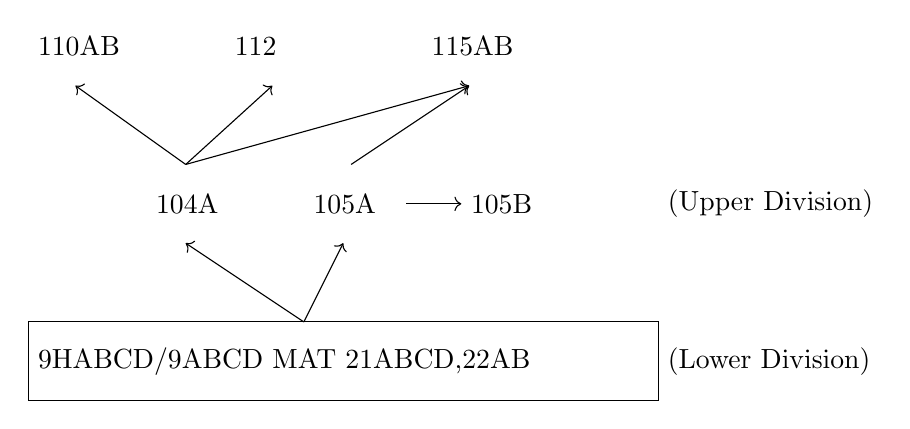
\begin{tikzpicture}

% 1st tier:
\node[right] at (0,0.5) {9HABCD/9ABCD MAT 21ABCD,22AB};
\draw (0,0) coordinate(X) -- ++(0,1) -- ++(8,0) |- (X);

\node[right] at (8,0.5) {(Lower Division)};

\draw[->] (3.5,1) --(2,2);
\draw[->] (3.5,1) --(4,2);

% 2nd tier:
\node[right] at (1.5,2.5) {104A};
\node[right] at (3.5,2.5) {105A};
\node[right] at (5.5,2.5) {105B};

\node[right] at (8,2.5) {(Upper Division)};


\draw[->] (4.8,2.5) --(5.5,2.5);
\draw[->] (2,3) --(0.6,4);
\draw[->] (2,3) --(3.1,4);
\draw[->] (2,3) --(5.6,4);

\draw[->] (4.1,3) --(5.6,4);

% 3rd tier:
\node[right] at (0,4.5) {110AB};
\node[right] at (2.5,4.5) {112};
\node[right] at (5,4.5) {115AB};

\end{tikzpicture}

\caption{\label{fig:prereqs} The prerequisite structure of required
  non-elective theoretical physics and math courses of the physics BS
  major.  Internal prerequisite structure of lower division coursework
  is not shown.  For clarity, only the most advanced prerequisites for
  each course are indicated.}
\end{center}
\end{figure}

An overview of the prerequisite structure of the core theoretical
physics courses is shown in Fig.~\ref{fig:prereqs}.  PHY 104A is the
major bottleneck in our program, as it requires the most advanced
material from the first tier (MAT 22B) but is required for every
course in the upper tier.  The committee spent a great deal of time
considering different ways to relieve or accommodate this bottleneck
but in the end decided two offerings is the only effective way to
achieve the goals of this proposal.  This stems from the fact that
incoming transfer students must start on 104A immediately upon arrival
in fall to complete the remaining upper division courses in two years,
but sophomores finishing 9HD in the fall are not generally ready to
take 104A until the spring.

The most important changes to the prerequisite structure in the proposal are:
\begin{itemize}
\item The 9 and 9H prerequisites have been updated to better reflect the current policy actually enforced.
\item PHY 112 does not require 115A anymore, it is taught at a level where 104A and PHY 9A-D suffice.  
\item PHY 110A does not require 105A anymore. 
\item PHY 105B requires 40, so that computational examples can be used in this course if the instructor chooses.
\item PHY 80 adds 40 as a prerequisite.
\item PHY 122A/B adds a 115A prerequisite, which was implicit when
  115A was a prerequisite for 112.  Both 112 and 115A are allowed to
  be concurrent, although that will never happen unless we add a fall
  offering of 122A/B.
\item The 116ABC sequence is replaced with independent courses 117 and
  118 which each have 80 as a prerequisite.

\end{itemize}
The new prerequisite structure is considerably more flexible.  In the
junior year of Tables~\ref{tbl:proposed-nonhonors} and
\ref{tbl:proposed-transfers} missing or failing 104A or 105A
jeopardizes a timely graduation, but instructor permission from one
course (110A or 115A) will allow the student to proceed on schedule.
The situation in Table~\ref{tbl:proposed-honors} is even more
forgiving.

\newpage

\section{Proposed BS with Specialization in Astrophysics}
The astrophysics specialization requires updates to the prerequisites
for PHY 151-158, mainly to accommodate the new schedule which offers
PHY 105A in the winter and to add PHY 40 as a new required course.  The
astrophysics specialty courses now include 158, for a total of five,
from which four are chosen.  Limits on the number of units preclude
including PHY 45, and the related lab courses, to the program.
However, the PHY 151-158 courses have already begun to include
extensive computational physics directly related to astrophysics.

The proposed required courses for the astrophysics specialization are presented in
Tables~\ref{tbl:prep-astro-applied} and \ref{tbl:depth-astro}.  To avoid
version conflicts, some information in Tables \ref{tbl:prep} and
\ref{tbl:depth} is not duplicated in these tables.  Example schedules are presented
in Table~\ref{tbl:proposed-astro}.

\captionof{table}{\label{tbl:prep-astro-applied}Preparatory Subject Matter:  Astrophysics, Applied Physics, and AB.}
\noindent
\vskip 0.25cm
\begin{center}
Units:  48-50. *: recommended.\\
\begin{tabular}{|lll|}
\hline
Course & & Units \\
\hline
MAT & 21A & 4 \\  
    & 21B & 4 \\ 
    & 21C & 4 \\ 
    & 21D & 4 \\
\hline
\hline
    & one of: & \\
\hline
MAT & 22A & 3 \\
    & 27A & 3 \\
    & 67  & 4 \\
\hline
\hline
MAT & 22B & 3 \\ 
    & or: & \\
MAT & 27B & 3 \\ 
\hline
\hline
PHY & 9A & 5 \\  
    & 9B & 5 \\  
    & 9C & 5 \\  
    & 9D & 4 \\  
\hline
&or&\\
\hline
PHY & 9HA & 5 \\  
    & 9HB & 5 \\  
    & 9HC & 5 \\  
    & 9HD & 5 \\  
\hline
\hline
PHY & 40   & 3 \\
    & 80   & 4 \\ 
    & 185* & 1 \\ 
    & 190* & 1 \\ 
\hline
\end{tabular}
\end{center}

\newpage
\captionof{table}{\label{tbl:depth-astro}Depth Subject Matter: Astrophysics}
\noindent
\vskip 0.25cm
Units:  60-64. *: recommended, $^\#$: not offered every year, $\parallel$: concurrently.\\
\begin{tabular}{|llllll|}
\hline
Course & & Units & Offered & Prereqs & Name \\
\hline
AST & 25* & 4 & & & \\ 
PHY & 104A & 4 & & & \\ 
    & 105A & 4 & & & \\
    & 108  & 3 & S & 9D/9HD & Optics \\  
    & 108L & 1 & S & $\parallel$108 & Optics Laboratory \\  
    & 110A & 4 & & & \\
    & 110B & 4 & & & \\
    & 112  & 4 & & & \\    
    & 115A & 4 & & & \\
    & 115B & 4 & & & \\
\hline
\hline
PHY & 157 & 4 & S$^\#$ & (Same as 122A/B) & Astronomy Instrumentation and \\  
    &     &   &     & & Data Analysis Lab\\  
\hline
    & or & & & & \\
\hline
PHY & 122A/B & 4 & & & Advanced Physics Laboratory \\  
\hline
\hline
 & Choose four of & & & \\
\hline
PHY & 151 & 4 & F$^\#$ & $\parallel$40,$\parallel$104A & Stellar Structure and Evolution \\ 
    & 152 & 4 & F$^\#$ & $\parallel$40,$\parallel$104A & Galactic Structure and \\
    &     &   &     &           & the Interstellar Medium\\
    & 153 & 4 & W$^\#$ & 40,104A,$\parallel$105A & Extragalactic Astrophysics\\  
    & 156 & 4 & W$^\#$ & 40,104A,$\parallel$105A & Introduction to Cosmology\\ 
    & 158  & 4 & S$^\#$ & 40,104A,105A & Galaxy Formation \\ 
\hline
 & Any two of & & & & : \\
\hline 
PHY & 105B & 4 &  &  & \\ 
    & 117 & 4 &  &  & \\  
    & 118 & 4 &  &  & \\  
    & 129A & 4 &  &  & \\  
    & 130A & 4 &  &  & \\  
    & 130B & 4 &  &  & \\  
    & 150  & 4 &  &  & Special Topics\\  
    & 154  & 4 & S$^\#$ & 40,105B,110B,115A & Astro. Appl. of Phys. \\
    & 155  & 4 & W   & 104A,105B,110A & General Relativity \\ 
GEL & 163  & 4 &  &  & Planetary Geology and Geophysics\\ 
 & At most one of &  &  &  & \\ 
PHY & 194HAB & 8 &  &  & Special Study for Honors Students\\ 
    & 195  & 5 &  &  & Senior Thesis\\
    & 198  & 3+ &  &  & Directed Group Study\\ 
    & 199  & 3+ &  &  & Special Study for Adv. Undergrads.\\ 
\hline
\end{tabular}\\
\vskip 0.25cm
\noindent
PHY 108 has alternative prerequisites (PHY 7C and 21D)
intended for non-majors.  PHY 150 must be an astro topic and requires
prior department approval.\\
\noindent
{\bf Total Units:} 108-114 \\

\newpage
\captionof{table}{An example schedule for the junior and senior year of an
  astrophysics major.  Physics course numbers are shown unless
  otherwise indicated.  Courses in italics are electives.  In most
  cases, the 9D requirement is satisfied before the junior year. The
  upper table starts with PHY 151 and the lower with 152.}
  \label{tbl:proposed-astro}
\begin{center}
\begin{tabular}{|l|l|l|l|}
\hline
Year      & Fall    & Winter & Spring \\
\hline
Junior    & 40         & 105A     & 80 \\
          & 104A       & 110A     & 110B \\
          & 151$^\#$   & 153$^\#$ & {\it 105B/150} \\         
          & (9D)       &             &  \\         
\hline
Senior   & 115A     & 115B & 108+L\\
         & 152$^\#$ & 156$^\#$ & 157/122A/B \\
         & 112   & {\it 130A/155/GEL 163} & {\it 158$^\#$/129A/130B} \\
\hline 
\end{tabular}

\vskip 0.5 cm

\begin{tabular}{|l|l|l|l|}
\hline
Year      & Fall    & Winter & Spring \\
\hline
Junior    & 40         & 105A     & 80 \\
          & 104A       & 110A     & 110B \\
          & 152$^\#$   & 156$^\#$ & {\it 105B/158$^\#$} \\         
          & (9D)       &             &  \\         
\hline
Senior   & 115A     & 115B & 108+L\\
         & 151$^\#$ & 153$^\#$ & 157/122A/B \\
         & 112   & {\it 130A/155/GEL 163} & {\it 154$^\#$/129A/130B} \\
\hline 
\end{tabular}
\vskip 0.5cm
\end{center}

\newpage
\section{Proposed Applied Physics Majors}

The applied physics majors overlap significantly with the physics
major, and so most of the updates already proposed apply directly to
the applied physics majors.  In this proposal, all applied physics
majors now require PHY 40, 45 (or an equivalent), 80, and at least one
computing lab (from 110L,112L, and 115L).  Most require two upper
division lab courses (from 122A/B, 117, 118) except where noted.

The applied physics majors typically require significant upper
division coursework outside of the physics department.  This proposals
makes several adjustments to the applied physics major requirements
which remove required courses that are no longer offered regularly, or
include a prohibitively large number of prerequisites.  The proposed
requirements take advantage of new relevant course offerings, by
giving students more options to choose from, offering greater
flexibility.

The applied physics majors (excluding chemical physics) require the
preparatory courses in Table~\ref{tbl:prep-astro-applied} and the
depth courses listed in Table~\ref{tbl:depth-applied}.  Together,
these required courses account for 72-74 units, leaving 38 units for
concentration courses as detailed in the following tables.  This
proposal includes modifications to all of the applied physics majors:
\begin{itemize}

  \item The Computational Physics major does not require PHY 45 and ECS
  36B will satisfy the prerequisite for the computing labs.  The
  elective choices from the Computer Science and Engineering
  department have been extended.  See Table~\ref{tbl:computational}.

\item The Physical Electronics major does not include 117 and 118 as
  part of the upper division lab requirement, only 122A/B is required.
  The major instead includes a large amount of electronics from the
  Electrical and Computer Engineering department.  Due to unit limits,
  only one computational lab is required.  See
  Table~\ref{tbl:electronics}.  An example schedule is presented in
  Table~\ref{tbl:electronics-two-year}.

\item The Materials Science major is renamed Materials Physics, and
  the elective choices have been extended.  Students may now use a
  Material Science and Engineering lab course as one of their required
  upper division lab courses.  See Table~\ref{tbl:materials}.

\item In the past, the Atmospheric Physics major required the Physical
  and Chemical Oceanography course (GEL 150A), which now has extensive
  prerequisites that would exceed the unit limit.  The Oceanography
  thrust of this course has been relocated to the electives, including
  the more easily obtained (GEL 116N).  The list of Atmospheric
  Physics electives has been extended.  See
  Table~\ref{tbl:atmospheric}.

\item The Physical and Chemical Oceanography course (GEL 150A) is not
  offered every year and now has extensive prerequisites.  Therefore,
  the Physical Oceanography major might not be achievable in two years
  for students that have not already satisfied these prerequisites.
  The prerequisites for reaching GEL 150A are now included in the
  concentration courses.  See Table~\ref{tbl:oceanography}.
  Additional example schedules are provided in
  Tables~\ref{tbl:oceanography-two-year}-\ref{tbl:oceanography-four-year}.
  
\item The Chemical Physics major requires the courses listed in
  Tables~\ref{tbl:prep-astro-applied} and~\ref{tbl:chemical}.  An
  example schedule is presented in Table~\ref{tbl:chemical-two-year}.
  Both chemistry and physics have significant lower division
  coursework as prerequisite for upper division coursework.  The
  additional 15 units of lower division general chemistry course
  work required by this major limits the number of upper division
  courses that can be required.  This major features two paths, one
  featuring PHY 112, 115AB, 140AB and the other featuring CHE 110ABC
  128AB.  The latter choice relies on the treatment of quantum
  mechanics and thermodynamics provided by our colleagues in the
  chemistry department.  This major requires 6 units of upper division
  lab work in chemistry or physics.
\end{itemize}
Some of the majors might benefit from further revisions, which we plan
to pursue once we have experience with the significant changes already
proposed here.  For example, it would be helpful if PHY 115AB were
listed as an alternative prerequisite for CHE 110B.

\captionof{table}{\label{tbl:depth-applied} Depth subject matter for
  all applied physics majors excluding chemical physics.}
\noindent
\vskip 0.25cm
\begin{center}
\begin{tabular}{|lll|}
\hline
Course & & Units \\
\hline
PHY & 104A   & 4 \\  
    & 105A   & 4 \\ 
    & 110A   & 4 \\ 
    & 110B   & 4 \\
    & 112    & 4 \\
    & 115A   & 4 \\ 
\hline
\end{tabular}
\end{center}

\newpage
\captionof{table}{\label{tbl:computational}Computational Physics}
\vskip 0.25cm
\noindent
{\bf Additional Preparatory Courses:  }\\
Units:  12 units. *: recommended, $^\#$: not offered every year, $\parallel$: concurrently.\\
\begin{tabular}{|llllll|}
\hline
Course & & Units & Offered & Prereqs & Name \\
\hline
ECS & 36A  & 4 & FWS & & Programming and Problem Solving\\
    & 36B  & 4 & FWS & & Software Dev. and OOP in C++\\
    & 36C  & 4 & FWS & & Data Structures, Algorithms, and Programming\\
\hline
\end{tabular}\\
\vskip 0.25cm
\noindent
{\bf Concentration Courses:  }\\
Units:  18 units. *: recommended, $^\#$: not offered every year, $\parallel$: concurrently.\\
\begin{tabular}{|llllll|}
\hline
Course & & Units & Offered & Prereqs & Name \\
\hline
ECS & 122A & 4 & FWS & & Algorithm Design \& Analysis\\
\hline
\hline
    & Choose two of & & & & \\
\hline
PHY    & 110L & 1 & & & \\
    & 115L & 1 & & & \\
    & 112L & 1 & & & \\
\hline
\hline
    & Choose one of & & & & \\
\hline
ECS & 120  & 4 & FWS & & Theory of Computation \\
    & 122B & 4 & WS  & & Algorithm Design \& Analysis \\
    & 132  & 4 & FWS & & Probability \& Stat Modeling \\
    & 171  & 4 & F   & & Machine Learning \\
\hline
\hline
    & Choose two of & & & & \\
\hline
PHY & 122A/B & 4 & & & \\
    & 117   & 4 & & & \\
    & 118   & 4 & & & \\
\hline
\end{tabular}\\
\vskip 0.25cm
\noindent
{\bf Additional Electives: (8 units)} Two courses for a total of at least 8 units of additional upper division coursework from ECS, MAT, or PHY.\\
{\bf Total Units:} 110-112\\
\vskip 0.25cm
\noindent
{\bf Example schedule:} In most cases, the 9D requirement is
satisfied before junior year, but an example including 9D is included.
Physics course numbers are shown unless otherwise indicated.  Courses
in italics are electives.\\
\begin{center}
\begin{tabular}{|l|l|l|l|}
\hline
Year      & Fall    & Winter & Spring \\
\hline
Junior    & ECS 36A    & ECS 36B      & ECS 36C \\
          & 40         & 105A         & 80 \\
          & 104A       & 110A         & 110B+L \\
          &            &              & (9D) \\         
\hline
Senior   & ECS 122A    & {\it ECS 122B} & {\it 122A} \\
         & 112+L       & {\it 118}      & \\
         & 115A        &                & \\
\hline
\end{tabular}
\end{center}

\newpage
\captionof{table}{\label{tbl:electronics}Physical Electronics }
\vskip 0.25cm
\noindent
{\bf Additional Preparatory Courses:  }\\
Units:  8 units. *: recommended, $^\#$: not offered every year, $\parallel$: concurrently.\\
\begin{tabular}{|llllll|}
\hline
Course & & Units & Offered & Prereqs & Name \\
\hline
ENG & 17     & 4 & & & Circuits I\\
PHY & 45     & 4 & & & \\
\hline
\end{tabular}\\
\vskip 0.25cm
\noindent
{\bf Concentration Courses:  }\\
Units:  30 units. *: recommended, $^\#$: not offered every year, $\parallel$: concurrently.\\
\begin{tabular}{|llllll|}
\hline
Course & & Units & Offered & Prereqs & Name \\
\hline
EEC & 100    & 4 & & ENG 17 & Circuits II\\
PHY & 115B*  & 4 & & & \\
    & 140A   & 4 & & & \\
    & 140B*  & 4 & & & \\
    & 122A/B & 4 & & & \\
\hline
\hline
    & Choose two of & & & & \\
\hline
PHY & 110L & 1 & & & \\
    & 115L & 1 & & & \\
    & 112L & 1 & & & \\
\hline
\hline
    & Choose four of & & & & \\
\hline
EEC & 110A  & 4 & & EEC 100, 140A$\parallel$& Electronic Circuits I \\
    & 110B  & 4 & & EEC 110A& Electronic Circuits II\\
    & 140A  & 4 & & ENG 17 & Principles of Device Physics I\\
    & 140B  & 4 & & EEC 140B & Principles of Device Physics II\\
    & 150   & 4 & & EEC 100 & Intro. to Signals \& Systems \\
    & 151   & 4 & & EEC 100 & Digital Signals \& Systems \\
\hline
\end{tabular}\\
\vskip 0.25cm
\noindent
{\bf Total Units:} 110-112\\

\captionof{table}{\label{tbl:electronics-two-year}Example two-year
  schedule for Physical Electronics major: In most cases, the PHY 9D
and ENG 17 requirements are satisfied before the junior year, but the
first example shows how those courses can be accommodated.  A
particular feature of this major is the ability to take graduate
courses in the senior year.  Physics course numbers are shown unless
otherwise indicated.  Courses in italics are electives.}
\begin{center}
\begin{tabular}{|l|l|l|l|}
\hline
Year      & Fall    & Winter & Spring \\
\hline
Junior    & (ENG 17)   & EEC 100    & (9D)\\
          & 40         & 45         & 80 \\
          & 104A       & 110A       & 110B+L \\
          &            & 105A       & \\         
\hline
Senior   & 112+L          & 140A             & 122A/B \\
         & 115A           & {\it EEC 110A}   & {\it EEC 110B} \\
         & {\it EEC 140A} & {\it EEC 150A}   & {\it EEC 245/249}\\
\hline
\end{tabular}
\end{center}

\newpage
\captionof{table}{\label{tbl:materials}Materials Physics}
\vskip 0.25cm
\noindent
{\bf Additional Preparatory Courses:  }\\
Units:  8 units. *: recommended, $^\#$: not offered every year, $\parallel$: concurrently.\\
\begin{tabular}{|llllll|}
\hline
Course & & Units & Offered & Prereqs & Name \\
\hline
PHY & 45     & 4 & & & \\
ENG & 45     & 4 & FWS & & Properties of Materials \\
\hline
\end{tabular}\\
\vskip 0.25cm
\noindent
{\bf Concentration Courses:  }\\
Units:  30-34 units. *: recommended, $^\#$: not offered every year, $\parallel$: concurrently.\\
\begin{tabular}{|llllll|}
\hline
Course & & Units & Offered & Prereqs & Name \\
\hline
PHY & 115B   & 4 & & & \\
    & 140A   & 4 & & & \\
    & 140B   & 4 & & & \\
    & 110L & 1 & & & \\
    & 115L & 1 & & & \\
    & 112L & 1 & & & \\
\hline
\hline
    & Choose two of & & & & \\
\hline
EMS & 162     & 4 & W & & Structure \& Characterization \\
    & 160+164 & 7 & F+W & & Thermo+Kinetics \\
    & 170     & 4 & S & & Sustainable Energy \\ 
    & 172     & 4 & F & & Smart Materials \\
    & 174     & 4 & S & & Mech. Behavior of Materials\\
    & 180     & 4 & F & & Materials in Eng. Design\\
\hline
\hline
    & Choose two of & & & & \\
\hline
PHY & 122A/B & 4 & & & \\
    & 117   & 4 & & & \\
    & 118   & 4 & & & \\
    & at most one of & & & & \\
EMS & 162L   & 3 & W & & Structure \& Characterization Lab\\
    & 170L   & 3 & S & & Sustainable Energy Lab \\
    & 172L   & 3 & F & & Smart Materials Lab \\
    & 174L   & 3 & S & & Mech. Behavior of Materials Lab \\
\hline
\end{tabular}\\
\noindent
{\bf Total Units:} 110-116 \\

\noindent
{\bf Example schedule:} In most cases, the PHY 9D and ENG 45 requirement is
satisfied before the junior year, but an example including these courses is
shown.  Physics course numbers are shown unless otherwise indicated.
Courses in italics are electives.
\begin{center}
\begin{tabular}{|l|l|l|l|}
\hline
Year      & Fall    & Winter & Spring \\
\hline
Junior    & 40         & 45           & 80 \\
          & 104A       & 110A         & 110B+L \\
          & (ENG 45)   & 105A         & (9D) \\         
\hline
Senior   & 112+L          & 140A   & 140B \\
         & 115A           & 115B+L & 122A \\
         & {\it EMS 180}  & 118   & {\it EMS 174} \\
\hline
\end{tabular}
\end{center}


\newpage
\captionof{table}{\label{tbl:atmospheric}Atmospheric Physics}
\vskip 0.25cm
\noindent
{\bf Additional Preparatory Courses:  }\\
Units: 11 units. *: recommended, $^\#$: not offered every year, $\parallel$: concurrently.\\
\begin{tabular}{|llllll|}
\hline
Course & & Units & Offered & Prereqs & Name \\
\hline
PHY & 45     & 4 &     & & \\
GEL & 50     & 3 & FWS & & Physical Geology \\
ATM & 60     & 4 & F   & & Intro. to Atmospheric Sci. \\
\hline
\end{tabular}\\
\vskip 0.25cm
\noindent
{\bf Concentration Courses:  }\\
Units:  27-29 units. *: recommended, $^\#$: not offered every year, $\parallel$: concurrently.\\
\begin{tabular}{|llllll|}
\hline
Course & & Units & Offered & Prereqs & Name \\
\hline
ATM & 120    & 4 & F   & ATM 60$\parallel$   & Atmos. Thermo. and Cloud Physics \\
    & 121A   & 4 & W   & ATM 120  & Atmospheric Dynamics \\
    & 121B   & 4 & S   & ATM 121A & Atmospheric Dynamics \\
\hline
\hline
    & Choose one of & & & & \\
\hline
PHY & 110L   & 1 & & & \\
    & 115L   & 1 & & & \\
    & 112L   & 1 & & & \\
\hline
\hline
    & Choose two of & & & & \\
\hline
PHY & 122A/B & 4 & & & \\
    & 117   & 4 & & & \\
    & 118   & 4 & & & \\
\hline
\hline
    & Choose two of & & & & \\
\hline
PHY  & 105B   & 4 & & & \\
     & 105C   & 4 & $^\#$  &             & Continuum Mechanics\\
GEL  & 116N   & 3 & S  & GEL 50      & Oceanography\\
     & 150A   & 4 & S$^\#$ & GEL 116N,55 & Physical and Chemical Oceanography\\
     & 150B   & 3 & W  & GEL 50      & Geological Oceanography\\
ATM  & 124    & 3 & F  & ATM 60      & Meteorological Instruments \& Observations \\
     & 128    & 4 & W  & ATM 60      & Radiation and Satellite Meteorology \\
     & 158    & 4 & S  & ATM 121A    & Boundary-Layer Meteorology \\
\hline
\end{tabular}\\
\vskip 0.25cm
\noindent
{\bf Total Units:} 110-114 \\

\noindent
{\bf Example schedule:} In most cases, the PHY 9D and GEL 50 are taken
before the junior year, but an example including these courses is
shown.  Physics course numbers are shown unless otherwise indicated.
Courses in italics are electives.
\begin{center}
\begin{tabular}{|l|l|l|l|}
\hline
Year      & Fall    & Winter & Spring \\
\hline
Junior    & 40         & 45           & 80 \\
          & 104A       & 105A         & {\it 105B} \\
          & ATM 60     & 110A         & 110B \\
          & (9D)       & (GEL 50)     & \\
\hline
Senior   & ATM 120       & ATM 121A     & ATM 121B \\
         & 112+L         & 118          & 122A \\
         & 115A          &              & {\it ATM 128}\\
\hline
\end{tabular}
\end{center}

\newpage
\captionof{table}{\label{tbl:oceanography}Physical Oceanography}
\vskip 0.25cm
\noindent
{\bf Additional Preparatory Courses:  }\\
Units:  15 units. *: recommended, $^\#$: not offered every year, $\parallel$: concurrently.\\
\begin{tabular}{|llllll|}
\hline
Course & & Units & Offered & Prereqs & Name \\
\hline
CHE  & 2A     & 5 & FW  & & \\
PHY  & 45     & 4 &     & & \\
GEL  & 50     & 3 & FWS & & Physical Geology \\
     & 55     & 3 & F      & CHE 2A & Intro. to Geochemistry\\
ATM  & 60*    & 4 & F   & & Intro. to Atmospheric Sci. \\
\hline
\end{tabular}\\
\vskip 0.25cm
\noindent
{\bf Concentration Courses:  }\\
Units:  23-25 units. *: recommended, $^\#$: not offered every year, $\parallel$: concurrently.\\
\begin{tabular}{|llllll|}
\hline
Course & & Units & Offered & Prereqs & Name \\
\hline
GEL  & 116N   & 3 & S      & GEL 50          & Oceanography\\
     & 150A   & 4 & S$^\#$ & GEL 116N,55 & Physical and Chemical Oceanography\\
\hline
    & Choose two of & & & & \\
\hline
PHY  & 110L & 1 & & & \\
     & 112L & 1 & & & \\
     & 115L & 1 & & & \\
\hline
\hline
    & Choose two of & & & & \\
\hline
PHY & 122A/B & 4 & & & \\
    & 117   & 4 & & & \\
    & 118   & 4 & & & \\
\hline
\hline
    & Choose two of & & & & \\
\hline
PHY  & 105B  & 4 & & & \\
     & 105C  & 4 & S$^\#$ & & Continuum Mechanics \\
ATM  & 115   & 3 & S   & ATM 60 & Hydroclimatology \\
     & 116   & 3 & F   & & Modern Climate Change \\
     & 120   & 4 & F   & ATM 60$\parallel$ & Atmos. Thermo. and Cloud Physics \\
GEL  & 150B  & 3 & W & GEL 50 & Geological Oceanography\\
\hline
\end{tabular}\\
\vskip 0.25cm
\noindent
{\bf Total Units:} 110-114\\
{\bf Note: } For transfer students arriving in their junior year, this
degree may not be possible to complete in two years.  Students should
seek instructor permission to take GEL 150A alongside 116N prerequisite if
it is offered in their junior year.\\

\newpage

\captionof{table}{\label{tbl:oceanography-two-year}Example two-year
  schedule for Physical Oceanography major.  In most cases, the PHY
  9D, CHE 2A, and GEL 50 requirements will be satisfied before the
  junior year, but an example including these courses is shown.
  Physics course numbers are shown unless otherwise indicated.
  Courses in italics are electives.}
\vskip 0.25cm
\begin{center}
\begin{tabular}{|l|l|l|l|}
\hline
Year      & Fall    & Winter & Spring \\
\hline
Junior    & 40         & 45           & 80 \\
          & 104A       & 105A         & 110B+L \\
          & (CHE 2A)   & 110A         & GEL 116N \\
          & (9D)       & (GEL 50)     &  \\
\hline
Senior   & GEL 55      & {\it GEL 150B}     & GEL 150A \\
         & 112+L       & {\it 118}         & {\it 122A}  \\
         & 115A        &              & \\
\hline
\end{tabular}


\captionof{table}{\label{tbl:oceanography-two-year-b}Example two-year
  schedule for Physical Oceanography major: This schedule assumes
  student took CHE 2A, GEL 50, and PHY 9D before the Junior year, and student
  receives instructor permission to take GEL 150A concurrently with GEL
  116N.  Physics course numbers are shown unless otherwise indicated.
  Courses in italics are electives.}
\vskip 0.25cm
\begin{center}
\begin{tabular}{|l|l|l|l|}
\hline
Year      & Fall    & Winter & Spring \\
\hline
Junior    & 40         & 45           & 110B \\ 
          & 104A       & 105A         & GEL 116N \\ 
          & GEL 55     & 110A         & GEL 150A \\
\hline
Senior   & 80          & {\it 118}      & {\it 122A}  \\
         & 112+L       & {\it GEL 150B} & \\
         & 115A        &                & \\
\hline
\end{tabular}
\end{center}
\captionof{table}{\label{tbl:oceanography-four-year}Example four-year
  schedule for Physical Oceanography major.  Physics course numbers are
  shown unless otherwise indicated.  Courses in italics are electives.
  If GEL 150A is not offered in junior year, it can be taken in senior
  year.}
\vskip 0.25cm
\begin{tabular}{|l|l|l|l|}
\hline
Year      & Fall    & Winter & Spring \\
\hline
Freshman  & MAT 21A  & MAT 21B  & MAT 21C \\
          & CHE 2A   & GEL 50   & 9A \\
\hline
Sophomore & MAT 21D  & MAT 22A  & MAT 22B \\ 
          & 9B       & 9C       & 9D \\
          & GEL 55   &          & GEL 116N \\
\hline
Junior    & 40       & 45       & 80\\
          & 104A     & 110A     & 110B+L\\
          &          & 105A     & GEL 150A \\         
\hline
Senior   & 115A      & {\it 118}     & {\it 122A}  \\
         & 112+L     & {\it GEL 150B}          & \\
\hline 
\end{tabular}

\end{center}

\newpage
\captionof{table}{\label{tbl:chemical}Chemical Physics}
\vskip 0.25cm
\noindent
{\bf Additional Preparatory Courses:  }\\
Units:  19 units. *: recommended, $^\#$: not offered every year, $\parallel$: concurrently.\\
\begin{tabular}{|llllll|}
\hline
Course & & Units & Offered & Prereqs & Name \\
\hline
\hline
CHE  & 2A      & 5 & FW & & General Chemistry \\
     & 2B      & 5 & WS & & General Chemistry \\
     & 2C      & 5 & FS & & General Chemistry \\
PHY  & 45      & 4 & & & \\
\hline
\end{tabular}\\
\noindent
{\bf Concentration Courses:  }\\
Units:  43-45 units. *: recommended, $^\#$: not offered every year, $\parallel$: concurrently.\\
\begin{tabular}{|llllll|}
\hline
Course & & Units & Offered & Prereqs & Name \\
\hline
PHY & 104A     & 4 & & & \\  
    & 105A     & 4 & & & \\ 
    & 110A     & 4 & & & \\ 
    & 110B     & 4 & & &\\    
CHE & 124A     & 3 & & & Inorganic Chemistry\\
\hline
\hline
PHY  & 115A   & 4 & & & \\
     & 115B   & 4 & & & \\
     & 112    & 4 & & & \\
     & 140A   & 4 & & & \\
     & 140B*   & 4 & & & \\
\hline
& Or: &&&& \\
\hline
CHE  & 110A   & 4 & & & Physical Chemistry: Intro to QM \\
     & 110B   & 4 & & & Physical Chemistry: Atoms and Molecules \\
     & 110C   & 4 & & & Physical Chemistry: Thermodynamics \\
     & 128A   & 4 & & & \\
     & 128B*   & 4 & & & \\
PHY  & 115A*  & 4 & & & \\
     & 112*   & 4 & & & \\
\hline
\hline
& Choose two of: &&&& \\
\hline
PHY  & 110L  & 1 & & & \\
     & 112L  & 1 & & & \\
     & 115L  & 1 & & & \\
\hline
& 6 or more units: & & & & \\
PHY & 122A/B & 4 & & & \\
    & 117   & 4 & & & \\
    & 118   & 4 & & & \\
CHE & 105    & 4 & & & Analytical \& Physical Chemical Methods \\
    & 115    & 4 & & & Instrumental Analysis \\
    & 124L   & 2 & & & Laboratory Methods in Inorganic Chemistry \\
    & 129A   & 2 & & & Organic Chemistry Laboratory \\
    & 129B   & 2 & & & Organic Chemistry Laboratory \\
    & 129C   & 2 & & & Organic Chemistry Laboratory \\
\hline
\end{tabular}\\
\noindent
{\bf Total Units:} 110-114 \\

\newpage
\captionof{table}{\label{tbl:chemical-two-year}Example two-year
  schedule for the chemical physics major.  Physics course numbers are
  shown unless otherwise indicated.  Courses in italics are electives.
  In most cases, the PHY 9D and CHE 2 requirements are satisfied
  before the junior year, but an example including these courses is
  shown.  }
\vskip 0.25cm
\begin{center}
\begin{tabular}{|l|l|l|l|}
\hline
Year      & Fall    & Winter & Spring \\
\hline
Junior    & (CHE 2A)   & (CHE 2B)     & (CHE 2C) \\
          & 40         & 45           & 80 \\
          & 104A       & 110A         & 110B+L \\
          & (9D)       & 105A         & \\

\hline
Senior   & 112+L         & 140A       & 140B\\
         & 115A          & 115B       & 122A\\
         & CHE 124A      & 118       &  \\
\hline
\end{tabular}
\end{center}


\newpage
\captionof{table}{\label{tbl:geophysics} Geological Physics}
\vskip 0.25cm
\noindent
{\bf Additional Preparatory Courses:  }\\
Units: 13 units. *: recommended, $^\#$: not offered every year, $\parallel$: concurrently.\\
\begin{tabular}{|llllll|}
\hline
Course & & Units & Offered & Prereqs & Name \\
\hline
PHY & 45     & 4 &     & & \\
GEL & 50     & 3 & FWS & & Physical Geology \\
    & 50L    & 2 &     & & Physical Geology Laboratory\\
ATM & 60     & 4 & F   & & Intro. to Atmospheric Sci. \\
\hline
\end{tabular}\\
\vskip 0.25cm
\noindent
{\bf Concentration Courses:  }\\
Units:  25-30 units. *: recommended, $^\#$: not offered every year, $\parallel$: concurrently.\\
\begin{tabular}{|llllll|}
\hline
Course & & Units & Offered & Prereqs & Name \\
\hline
    & Choose two of & & & & \\
\hline
PHY & 110L   & 1 & & & \\
    & 115L   & 1 & & & \\
    & 112L   & 1 & & & \\
\hline
\hline
    & Choose two of & & & & \\
\hline
PHY & 122A/B & 4 & & & \\
    & 117   & 4 & & & \\
    & 118   & 4 & & & \\
\hline
\hline
    & Choose five of & & & & \\
\hline
PHY  & 105B   & 4 & &  & \\
     & 105C   & 4 & &  & Continuum Mechanics\\
ATM  & 120    & 4 & F  & ATM 60    & Atmospheric Thermodynamics \& Cloud Physics \\
     & 121A   & 4 & F  & ATM 120   & Atmospheric Dynamics \\
     & 121B   & 4 & W  & ATM 121A  & Atmospheric Dynamics \\
GEL  & 116N   & 3 &    & & Oceanography\\
     & 146    & 3 &    & & Radiogenic Isotope Geochemistry \& Cosmochemistry \\
     & 150A   & 4 & S$^\#$ & GEL 116N,55 & Physical and Chemical Oceanography\\
     & 150B   & 3 & W  & GEL 50      & Geological Oceanography\\
\hline
     & incl at least two:  & & & & \\
\hline
GEL  & 161    & 3 & S$^\#$ & GEL 50 & Geophysical Field Methods \\
     & 162    & 3 & W$^\#$ & GEL 50 & Geophysics of the Solid Earth \\
     & 163    & 3 & F$^\#$ & GEL 50 & Planetary Geology \\
\hline
\end{tabular}\\
\vskip 0.25cm
\noindent
{\bf Total Units:} 110-117 \\

\noindent
{\bf Example schedule:} In most cases, the PHY 9D and GEL 50 are taken
before the junior year, but an example including these courses is
shown.  Physics course numbers are shown unless otherwise indicated.
Courses in italics are electives.
\begin{center}
\begin{tabular}{|l|l|l|l|}
\hline
Year      & Fall    & Winter & Spring \\
\hline
Junior    & 40         & 45           & 80 \\
          & 104A       & 105A         & 105B\\
          & ATM 60     & 110A         & 110B \\
          & (9D)       & (GEL 50+L)   & GEL 161\\
\hline
Senior   & 112+L       & ATM 121A     & 122A \\
         & 115A        & 118          & \\
         & ATM 120     & GEL 162      & \\
\hline
\end{tabular}
\end{center}



\newpage
\section{Proposed AB Physics Major}
\label{sec:ab}

The proposed requirements for the AB Physics major are listed in
Tables~\ref{tbl:prep-astro-applied} and \ref{tbl:ab-depth}.  To avoid
version conflicts, some information in Tables \ref{tbl:prep} and
\ref{tbl:depth} is not duplicated in these tables.

The college requirements for an AB degree include a cap of 80
units, of which at least 36 must be upper division.  This presents a
very fine needle to thread indeed!  The current AB Physics degree
requires 82 units, which was approved by the Education Policy
Committee in the past despite exceeding the cap.  This proposal
requires only 80 units for the AB.

The proposed AB Physics major only requires 32 units of upper division coursework, which
does not reach the required 36 unit minimum.  However, several
required lower-division courses, such as PHY 80 and PHY 45 include
significant prerequisites and are therefore quite nearly upper
division courses.  We will therefore ask for an exception to the 36
unit {\bf minimum} (our preference) or an exception to the 80 unit
{\bf maximum} (and require two instead of one elective upper division
courses in Table~\ref{tbl:ab-depth}).

\captionof{table}{\label{tbl:ab-depth}Depth Subject Matter}
\noindent
\vskip 0.25cm
\begin{center}
Units:  32. *: recommended, $\parallel$: concurrently.\\
\begin{tabular}{|lll|}
\hline
Course & & Units \\
\hline
PHY & 104A & 4 \\
    & 105A & 4 \\
    & 110A & 4 \\
    & 110B & 4 \\
    & 112  & 4 \\
    & 115A & 4 \\
\hline
\hline
PHY & 122A/B & 4 \\
\hline
    & At least one of & \\ 
\hline
PHY & 129A & 4 \\
    & 130A & 4 \\
    & 140A & 4 \\
    & 151 & 4 \\
    & 152 & 4 \\
    & 153 & 4 \\
    & 156 & 4 \\
    & 158 & 4 \\
\hline
\end{tabular}\\ \vskip 0.25cm
\end{center}
\noindent
{\bf Foreign Language:} The AB degree requires proficiency in a language other than English (15 units)\\
\noindent
{\bf Total Units:} 80-82 units, excluding language requirement.
\newpage
\section{Example Course Syllabi}
\label{sec:syllabi}

This section contains example syllabi for new courses and existing
courses impacted by this proposal.  The first paragraph for each
course is a brief description suitable for the course catalog, and is
generally much less specific than the details that follow.  This is to
allow some flexibility to maintain the course content within the
department without contradicting the course catalog.

Instructors are expected to satisfy the brief course description as
listed in the course catalog, but are not obliged to follow the
detailed example syllabi shown here.  However, many of these courses
are prerequisite courses, so instructors are expected to consider how
their course content decisions will impact downstream courses.

The specific computational tools (e.g. Scientific Python, C++) will
not be included in the course catalog description.  This is to allow
the department some flexibility to evolve independently over time.
However, the choice of tool set needs to be coordinated throughout the
department.  It would be extremely disruptive if the instructor for
PHY 40 or 45 made changes to the tool set without coordinating with
the rest of the department.  Specific details about the current
computational tool set will be publicly available on the department
website, including guidance for installation.

\vskip 1cm
\noindent
{\bf PHY 40 --- Introduction to Computational Physics (3):}
Introduction to programming with examples from numerical analysis and
computational physics. Introduction to modern tools used for
scientific analysis and computer algebra.

The language for this course will be Python/Anaconda, with some
symbolic manipulation via Mathematica or the developing Python
equivalent (SymPy).  The supported operating systems will be Windows,
MacOS, and Linux.  The course introduces the Python language and the
Scientific Python ecosystem in the context of an introduction to
numerical analysis.  The major topics of numerical analysis are
introduced with the most elementary of algorithms, for example
numerical integration via Newton-Cotes methods (e.g. Simpson's rule)
are covered, but Gaussian Quadrature methods are not.  The Scientific
Python tools, which generally implement more sophisticated algorithms,
can then be used with a basic understanding of how they work.  This
approach minimizes formal pedagogy, so that the students can learn by
coding themselves.  This course has no prerequisites, but most of the
elementary techniques are intuitively graphical.  For example,
Simpson's method of integration can be easily explained as estimating
the area under the curve.  Whenever possible, special cases with
analytic solutions are used to validate the numerical approach.

We find that students taking this as their first computing course are
not yet ready to complete computing exercises unsupervised.
Therefore, this course has nearly zero homework outside of the
schedule lecture and lab time.

There are a surprising large number of excellent textbooks, some dated
and many quite recent, in computational physics.  These syllabi use
Gezerlis for references when possible because the textbook is
available as a PDF from the UCD library.  Giordano is a particularly
excellent source for approachable problems.

The core course content is:
\begin{itemize}
\item Python language elements:  variables, conditionals, loops, input and output, and lists. Taught through a series of simple math problems: from arithmetic, geometric and Taylor series, to the quadratic equation. (6 hours)
\item Scientific Python ecosystem:  numpy, matplotlib, scipy including 1-D arrays, plotting, and numerical analysis tools.  Taught as encountered.
\item Fundamental limits to numerical analysis:  representation of numbers on computers, errors from approximation and round-off. (2 hours) [Gezerlis 2]
\item Differentiation:  Finite difference and error estimation, scipy tools. (2 hours) [Gezerlis 3.3]
\item Integration:  Newton-Cotes methods, scipy tools (2 hours) [Gezerlis 7.2]
\item Roots: bisection, Newton's method, secant method, scipy tools. (2 hours) [Gezerlis 5.2.4-5.2.6]
\item Monte Carlo: Quadrature, scipy tools (2 hours) [Gezerlis 7.7.2]
\item Ordinary Differential Equations:  Euler and Verlet/Leap frog methods, Mass on spring with damping, Euler-Cromer Kepler problem (5 hours) [Gezerlis 8.2, Giordano 4.1]
\item Computer Algebra (5 hours):  Mathematica or SymPy
\item Analytic solutions to special cases are calculated and used throughout the
  course to validate the numerical approach.
\end{itemize}
The time allocated for core material is generous, which should leave room for topical material.  Example topical approachable material:
\begin{itemize}
\item Cellular Automata:  Game of Life
\item Sorting:  Bubble sort, Merge Sort, scipy tools
\item Chaos:  Logistics Map, Period Doubling
\item Fractals: Mandelbrot Set
\item Fourier Series:  visualization for square wave
\item Simulating Musical Instruments (Giordano 11)
\end{itemize}

\vskip 1cm
\noindent
{\bf PHY 45 --- Computational Physics (4):}
Algorithms and programming techniques of computational physics
with applications from introductory physics.

This course builds on the programming, numerical analysis, and basic
computational physics techniques from PHY 40.  The algorithms and
problems considered in this course are more sophisticated, using
theoretical physics and mathematical concepts from PHY 9ABC, and MAT
21ABCD, and MAT 22A.  Students may take MAT 22B concurrently, so the
more challenging differential equation related material is left for
the second half of the course.

The core material is:
\begin{itemize}
\item C/C++ language elements: variables, conditionals, loops, input
  and output, arrays and pointers.  Taught through a series of
  computing tasks as in 40. (6 hours)
\item Continued use of Scientific Python, particularly for plotting
  and matrices.  Some problems will be solved twice: once in Python
  and once in C++.  Taught as encountered.
\item Matrices: Linear Algebra, Eigenvalues and Eigenvectors [Gezerlis 4] (3 hours)
\item Molecular Dynamics:  Direct Simulation [Giordano 9] (2 hours)
\item Monte Carlo Techniques: Pseudo-random Numbers, Inverse Transform Sampling, Importance Sampling, Random Walks [Gezerlis 7.7.1-7.7.4, Giordano 7] (3 hours)
\item Ordinary Differential Equations:  Runge-Kutta, Shooting Method [Gezerlis 8.2-3] (3 hours)
\item Partial  Differential Equations:  Diffusion, Relaxation  [Garcia 6,8] (3 hours)
\item Fourier Analysis:  Spectral methods [Gezerlis 6.4.1-6.4.3, Garcia 8.2] (4 hours)
\end{itemize}
This leaves plenty of time for topical problems, such as:
\begin{itemize}
\item Projectile motion with air resistance [Giordano 2.2] (ODEs)
\item Chaos in the Driven Nonlinear Pendulum [Giordano 3.2] (ODEs) 
\item Extensions to the Kepler problem:  precession and Kirkwood gaps [Giordano 4.3, 4.5 ] (ODEs)
\item Charged particle in a magnetic field via Runge Kutta  (ODEs)
\item Kinetic energy of particle in a box [Gezerlis 3.4] (Differentiation)
\item Normal modes of a mass/spring/pendulum system (Matrices)  
\item Eigenvalues of the Schr\"odinger equation [Gezerlis 4.5] (Matrices)
\item Shooting Method Solution to Schr\"odinger Equation [Giordano 10.2] (QM / ODE)
\item Relaxation Method for solving Laplace's Equation [Giordano 5.1] (EM / PDEs)
\item Manhattan Project, critical mass [Garcia 6.3] (Diffusion / PDEs)
\item Direct simulation of an Ideal Gas [Giordano 9] (SM / Molecular Dynamics)
\item Analytic solutions to special cases are calculated and used throughout the
  course to validate the numerical approach.
\end{itemize}  

\vskip 1cm
\noindent
{\bf PHY 80 --- Experimental Techniques (4):}
Experimental techniques. Design of circuits. Data analysis, sources of
noise, statistical and systematic uncertainties. Light sources,
detection, and measurement in basic optical systems.

PHY 80 uses Scientific Python for data analysis.  With PHY 40 added as
a prerequisite, this component can be more ambitious:
\begin{itemize}
\item Plotting and Curve fitting (Current focus)
\item Fourier Analysis: discrete sampled data and Shannon-Nyquist, periodogram (New)
\item Monte Carlo:  generating simulated experimental data. (Expand)
\item Machine Learning (Optional)
\end{itemize}

\newpage

\vskip 1cm
\noindent {\bf PHY 104A --- Introduction to Mathematical Methods in Physics (4):}
Introduction to the mathematics used in upper division physics
courses. Vector spaces, Fourier analysis, and partial differential
equations.

This course includes review of some material from MAT 21D and MAT
22AB, In particular, instructors teaching 104A should coordinate with
the instructor for 110A to ensure that vector calculus is being
adequately covered.  The amount of time devoted to review can be
adjusted in the fall and spring offerings to best suit the class
composition, which will be predominantly students from the PHY 9
series, including transfer students, in the fall, versus 9H students
in the spring.  Textbook: Mathematical Methods in the Physical
Sciences, 3rd Edition by Mary L. Boas.  It might be beneficial to
leave vector analysis until the end of course, as many students will
start 110A in the following quarter.  Note that treatment of Fourier
Transforms is restricted to the limit of the Fourier Series as the
period becomes infinite.

\begin{samepage}
Example coverage:
\begin{itemize}
\item Quick Review of Complex Numbers (Ch. 2) (as needed - 1.5 hour)
\item Quick Review of Sequences and Series, including Taylor (1.1-1.15) (as needed - 1.5 hour)
\item Linear Algebra (3.6-3.12,3.14,12.6) (6 hours)
\item Fourier Series and Transforms (7.1-7.12) (6 hours)
\item Dirac Delta Function ( 8.11) (1.5 hours)
\item Legendre Series (12.1-12.10) (3 hours)
\item Partial Differential Equations (Intro+13.2) (3 hours)
\item Series Solutions to PDEs (13.3-13.8) (3 hours)
\item Review of Vector Calculus (Ch. 6) (important for 110A - 3 hours)
\item Linearity and Dimensional Analysis (reinforced throughout course)
\end{itemize}
\end{samepage}

\vskip 1cm
\noindent {\bf PHY 104B --- Intermediate Methods of Mathematical Physics (4):}  
Continuation of 104A.  Contour Integration, Fourier Transforms, and other topics in Mathematical Physics.

This is more topical than PHY 104A, but some topics should be routinely covered:
\begin{itemize}
 \item Contour Integration (Ch. 14)
 \item Fourier Transforms
\end{itemize}
while others are at the discretion of the instructor:
\begin{itemize}
 \item Tensors (Ch. 10)
 \item Group Theory
 \item Green Functions
 \item Probability and Statistics (Ch. 15)
\end{itemize}


\vskip 1cm
\noindent {\bf PHY 105A ---  Classical Mechanics I (4):}
Principles and applications of Newtonian mechanics. Introduction to
Lagrangian and Hamiltonian mechanics.

The recommended textbook for this course is Morin plus supplementary
material to include Hamiltonian dynamics.  Hamiltonian dynamics must
be covered reliably in this course.  It cannot be postponed until PHY
105B, as not all students will take 105B before taking quantum mechanics.
\begin{itemize}
 \item Basic Problem Solving Techniques (Ch. 1) (reinforce throughout)
 \item Newtonian Mechanics (Ch. 2-3) (2 weeks)
 \item Oscillations (Ch 4) (1.5 weeks)
 \item Conservation of Energy and Momentum (Ch 4 )(1.5 weeks)
 \item Lagrangian Mechanics (1.5 week)
 \item Hamiltonian Mechanics (1.5 week)
\end{itemize}
   
\vskip 1cm
\noindent {\bf PHY 105B ---  Classical Mechanics II (4):}
Continuation of PHY 105A.  Lagrangian and Hamiltonian Mechanics,
Calculus of Variations, Conservation Laws, Non-inertial Frames,
Special Relativity.

This course goes beyond the material in Morin.  Reference text is
Marion and Thorton.  The core material which must be reliably covered
is:
\begin{itemize}
 \item Review of Calculus of Variations, Lagrangian and Hamiltonian Mechanics (Ch 6-7) 
 \item Gravity, Central Force Motion and Angular Momentum (Ch 5, 8)
 \item Non-inertial Frames (Ch 10) 
 \item Special Relativity (Ch 14)
\end{itemize}
That leaves time for additional topical material, for example:
\begin{itemize}
 \item Dynamics of a System of Particles, Collisions (Ch 9) 
 \item Rigid Body Dynamics (Ch 11)
 \item Continuous Systems and Waves (Ch 13)
\end{itemize}

\newpage

\vskip 1cm
\noindent {\bf PHY 110A --- Electricity and Magnetism I (4):}  
Theory of electrostatics, magnetostatics, electrodynamics and radiation.

The first quarter of 110 focuses on electrostatics and magnetostatics
(Griffiths 1-6).  An example schedule:
\begin{itemize}
\item Week 1: quick review on vector analysis, Coulomb's law, Gauss's law, electric potential (2.1,2.2, 2.3)
\item Week 2: electric energy, conductors, image method (Cartesian only) (2.4, 2.5, 3.2)
\item Week 3: Laplace's equation (Cartesian) (3.1, 3.3.1)
\item Week 4: Laplace's equation (spherical only), multipole expansion (3.3.2, 3.4)
\item Week 5: dipole in E, polarization, bound charge (4.1, 4.2)
\item Week 6: displacement field (4.3)
\item Week 7: review of Lorentz force, Bio-Savart, Ampere's law (5.1, 5.2, 5.3)
\item Week 8: magnetic potential, multipole expansion, dipole in B (5.4, 6.1)
\item Week 9: magnetization, bound current, H field (6.1, 6.2, 6.3)
\end{itemize}

\noindent {\bf PHY 110B --- Electricity and Magnetism II (4):}  
Theory of electrostatics, magnetostatics, electrodynamics and radiation.

The second quarter focuses on electrodynamics and radiation (Griffiths 7-12).
An example schedule:
\begin{itemize}
\item Week 1: motional EFM, Faraday's law (7.1, 7.2)
\item Week 2: inductance, magnetic energy, Maxwell equations (7.2, 7.3)
\item Week 3: conservation laws (8)
\item Week 4: plane wave, energy, momentum of a plane wave (9.1, 9.2)
\item Week 5: reflection and refraction, absorption and dispersion (only for insulating medium) (9.3, 9.4)
\item Week 6: retarded potential formulation (10.1-2)
\item Week 7: radiation from dipoles (11.1)
\item Week 8: review of Lorentz transformation and relativistic mechanics (12.1, 12.2)
\item Week 9: relativistic electrodynamics (12.3)
\end{itemize}
This version omits wave guides (9.5) and radiation from point charges
(11.2).  These topics could be included by spending less time on other
topics.
\newpage

\vskip 1cm
\noindent
{\bf PHY 110L --- Computational Physics Lab for Electricity and Magnetism (1):}
Applications of computational physics to problems from Electricity and
Magnetism.

This course, which has one hour of lecture per week, includes
extensive problems from numerical physics related to PHY 110AB, using
the techniques introduced in PHY 40 and 45.

See comments in Section~\ref{sec:computing} regarding workload for one
unit courses.  Example topics for assignments include:
\begin{itemize}
\item Variations of related problems from PHY 45.
\item Visualizing Electric and Magnetic fields (Gezerlis 1.7)
\item Multipole Expansion (Gezerlis 4.2)
\item Magnetic Fields produced by current distribution (Giordano 5.3-4)
\item Waves on a String: Spectral methods (Giordano 6.4)
\item Relaxation Method Solution to Laplace's Equation (Giordano 5.1-2, Garcia 8)
\item Fourier Analysis:  Spectral method (Garcia 8.2)
\item Waveguides
\item Analytic solutions to special cases are calculated and used throughout the
  course to validate the numerical approach.
\end{itemize}

\vskip 1cm
\noindent {\bf PHY 112 --- Thermodynamics and Statistical Mechanics (4):}  
Introduction to classical and quantum statistical mechanics and their connections with thermodynamics.

The reference text is ``Thermal Physics'' by Schroeder.  The core topics are:
\begin{itemize}
\item Energy in Thermal Physics (Chap 1)
\item Second Law of Thermodynamics (Chap 2)
\item Interactions and Implications (Chap 3)
\item Free Energy (Chap 5)
\item Boltzmann Statistics (Chap 6) (Target for midpoint of course)
\item Quantum Statistics (Chap 7) 
\end{itemize}

\vskip 1cm
\noindent
{\bf PHY 112L --- Computational Physics Lab for Statistical Mechanics (1):}
Applications of computational physics to problems from statistical mechanics.

This course, which has one hour of lecture per week, includes
extensive problems from numerical physics related to PHY 105A and 112,
using the techniques introduced in PHY 40 and 45.
% see also Garcia 11 when arrives

See comments in Section~\ref{sec:computing} regarding workload for one
unit courses.  Example topics for assignments include:
\begin{itemize}
\item Variations of related problems from PHY 45.
\item Testing the Stefan-Boltzmann Law (Gezerlis 6.6)
\item Mean Field Theory Solution to Ising Model (Giordano 8.2)
\item Metropolis Algorithm (Giordano 8.3)
\item Phase Transitions (Giordano 8.4-8.5)
\item Monte Carlo Simulation of Dilute Gas (Giordano 9.1) 
\item Melting (Giordano 9.2)
\item Protein Folding (Giordano 12.1)
\item Analytic solutions to special cases are calculated and used throughout the
  course to validate the numerical approach.
\end{itemize}



\vskip 1cm
\noindent
{\bf PHY 115A --- Quantum Mechanics I (4):}
Introduction to quantum mechanics.  The Schr\"odinger Equation, Hilbert
Space, Dirac Notation, position and momentum space representations,
stationary states, and applications.

The topics in this course (and PHY 115B) may be presented as a
historical progression or with spin first.  Both approaches are valid
but must be coordinated between both courses.  The reference text for
spin first is Townsend, and the reference for historical progression is
Griffith.  Either ordering provide a sufficient introduction to
quantum mechanics by the end of PHY 115A for majors that do not
require PHY 115B.

The core material for the Griffith-based progression is: 
\begin{itemize}
\item Wave functions and the Schr\"odinger equation (1.1-1.4) (2 hours)
\item Momentum, operators, uncertainty principle (1.5-1.6) (2 hours)
\item Stationary states, infinite square well (2.1-2.2) (4 hours)
\item Harmonic oscillator (2.3) (4 hours)
\item Free particle, momentum space; delta function potential (2.4) (3 hours)
\item Finite square wells; the scattering matrix (2.5-2.6) (3 hours)
\item The WKB approximation (9.1-9.2) (2 hours)
\item Linear algebra, Hilbert spaces, operators (3.1-3.3) (2 hours)
\item Dirac notation, Axioms of quantum mechanics, Uncertainty  (3.4-3.6) (2 hours)
\end{itemize}
This leaves some time for topical material:
\begin{itemize}
\item Two-state systems
\item Bell's inequality, EPR paradox, and hidden variables.
\end{itemize}

The core material for the Townsend-based progression is: 
\begin{itemize}
\item Basis states and matrix mechanics operators, eigenstates, and
  basis transformations.
\item Angular momentum eigenstates
\item Time evolution and the Schr\"odinger equation
\item Multiple spin states and entanglement: Bell states and EPR paradox
\item Density Matrix formalism: pure vs mixed states
\item Wave mechanics in 1D
\end{itemize}
This approach relies on students have a strong background in Linear Algebra, which must be reliably covered in PHY 104A.

\vskip 1cm
\noindent
{\bf PHY 115B --- Quantum Mechanics II (4):}
Continuation of PHY 115A.  Angular momentum and spin, central potentials and the hydrogen atom, perturbation theory and scattering.

The material covered in PHY 115B depends on the treatment in 115A: either Griffith-based or Townsend-based (spin first).

The material for the Griffith-based progression are:
\begin{itemize}
\item Review particle in a box and harmonic oscillator 
\item Angular momentum: algebraic methods and spherical harmonics
\item Bound states of central potentials: Hydrogen atom
\item Spin-orbit coupling and relativistic corrections
\item Time-independent perturbation theory
\item Time-dependent perturbation theory and scattering
\item Quantum field theory for scalar fields
\end{itemize}

The material for the Townsend-based progression are:
\begin{itemize}
\item Review angular momentum 
\item Particle in a box and quantum tunneling
\item Harmonic Oscillator
\item Translation and Rotation in 3D
\item Symmetries of 2-body problem 
\item Bound states of central potentials: Hydrogen atom
\item Time-independent perturbation theory
\item Time-dependent perturbation theory and scattering
\end{itemize}

The review topics are intended to cover the crucial material that would
otherwise be missed for students who took PHY 115A under a different
ordering.  This situation should be a rare occurrence: instructors tend
to teach for multiple years in a row, and students tend to take both
courses within the same year.

\vskip 1cm
\noindent
{\bf PHY 115L --- Computational Physics Lab for Quantum Mechanics (1):}
Applications of computational physics to problems from Classical and Quantum Mechanics.

This course, which has one hour of lecture per week, includes
extensive problems from numerical physics related to PHY 115A and 115B,
using the techniques introduced in PHY 40 and 45.

See comments in Section~\ref{sec:computing} regarding workload for one
unit courses.  Example topics for assignments include:
\begin{itemize}
\item Variations of related problems from PHY 45.
\item Symplectic Algorithms
\item Extremizing the Action (Gezerlis 5.6)
\item Solution of the Time-independent Schr\"odinger equation: 
  Harmonic oscillator, Lennard-Jones potential (Giordano 10.2).
\item Variational Quantum Monte Carlo (Giordano 10.4, Gezerlis 7.8)
\item Time-dependent Schr\"odinger equation:  reflection of wave packets (Giordano 10.5)
\item Spectral method solutions to Schr\"odinger equation.  (Giordano 10.7)
\item Matrix Representation of Interacting spin-half particles (Gezerlis 4.5)
\item Analytic solutions to special cases are calculated and used throughout the course to validate the numerical approach.
\end{itemize}





\vskip 1cm
\noindent
{\bf PHY 117 --- Physics Instrumentation with Analog and Digital Electronics (4):}  
Experimental and theoretical study of important electronic circuits
involving analog and digital components.  Feedback, amplifiers,
oscillators, noise, integrated circuits, digital logic, timers,
analog-to-digital and digital-to-analog converters.


{\bf Summary of Course Content:}
This course provides a theoretical understanding and practical
experience with the use of analog and digital electronics within the
context of instrumentation for physics experiments.

The lecture content is primarily in support of the lab activities.
The lab activities survey the essential devices used for physics
instrumentation, excluding passive compenents (resistors, capacitors,
and diodes) covered in PHY 80.  It excludes modern high-density
integrated circuits, such as FPGAs and CPUs, which are covered in PHY
118.  The lab topics include: transistors, operational amplifiers,
power amplifiers, schmitt triggers, oscillators, gates, flip-flops,
combinatorics, synchronous logic, and analog-to-digital and
digital-to-analog conversion.  There is also room for topical
interests of each instructor.  The lectures develop physics models for
each device which are used to calculate their theoretical behavior,
and discuss the ways in which each device contributes to physical
instrumentation.

{\bf Illustrative Reading:}
The Art of Electronics by Horowitz and Hill
Practical Electronics for Inventors by Scherz
Experiments in Modern Physics by Melissinos and Napolitano

{\bf Potential Course Overlap:} This course has substantial overlap
with many courses in electrical and computer engineering, most notably
EEC 110A, 110B, 140A, and 18.  However, this course is substantially
different from any of these courses.  Most importantly, this course
does not attempt to reach the level of mastery in electronic design
that an electrical engineer reaches through years of study and
practice.  Instead, this is a one quarter survey of the essential
analog and digital devices which a scientist is likely to encounter in
the context of instrumenting an experiment.  This course prepares
future scientists with a basic understanding of the operational
behavior of these devices which is needed for productive collaboration
with engineers to design experiments.  We do have an applied physics
major in electronic devices which attempts to reach the same level of
mastery as engineers in some of these topics.  Those students are
required to take coursework in EEC instead of taking PHY 117 or 118.



\vskip 1cm
\noindent 
{\bf PHY 118 --- Physics Instrumentation for Data Acquisition (4):}  
Experimental application of modern high density integrated circuits.
Automated data acquisition,  microprocessors, field programmable gate arrays.

{\bf Summary of Course Content:}
This course provides practical experience with using modern
high-density integrated circuits to develop custom data acquisition
circuits for physics experiments.

The lecture content is primarily in support of the lab activities,
which deploy FPGAs and microprocessors to create a scalar, function
generator, digital oscilloscope, and spectrum analyzier.  In order to
do so, students learn to write microprocessor code and high level
description code for FPGAs.  Students use their custom data
acquisition system to conduct experiments exploring physical
phenomemon such as radioactivity, muon decay, and johnson noise.  The
lectures further explore the role that data acquisition systems play
in modern physics experiments.

{\bf Illustrative Reading:}
A Verilog HDL Primer by Bhasker
FPGA Prototyping by VHDL Examples by Chu
Getting Started with Arudino by Banzi and Shiloh
Experiments in Modern Physics by Melissinos and Napolitano


{\bf Potential Course Overlap:} This course has substantial overlap
with many courses in electrical and computer engineering, most notably
EEC 170, 172, 180, and 181A/B.  However, this course is substantially
different from any of these courses.  Most importantly, this course
does not attempt to reach the level of mastery in electronic design
that an electrical engineer reaches through years of study and
practice.  Instead, this course covers the basics of programming
microprocessors and configuring FPGAs at a level sufficient to
instrument basic physics experiments.  This course prepares future
scientists with a basic understanding of the operational behavior of
these essential devices which is needed for productive collaboration
with engineers to design experiments.  We do have an applied physics
major in electronic devices which attempts to reach the same level of
mastery as engineers in some topics.  Those students are required to
take their electronics courses in EEC instead of taking PHY 117 or
118.

\newpage

\section{Implementation}
\label{sec:implementation}

Some aspects of this proposal involve changing the scheduling and
number of offerings of certain courses, which does not require campus
approval, and the department has already begun to implement those
changes in AY 2021-2022.  This first year implements changes for
juniors and earlier, while allowing seniors to finish under the
current schedule.  In the tables below, only the courses directly
impacted by this proposal are shown.

Changes to the curriculum are tracked in the integrated curriculum
management system (ICMS).  Each proposed change is approved at the
level of UGCC/Vice-Chair, College, and then the Senate Committee on
Courses of Instruction (COCI).

All departments with courses that include prerequisites that would be
impacted have already been contacted (Electrical and Computer
Engineering ).  We will also reach out to the departments hosting
courses for our applied majors: they won't need to make any changes
but they might appreciate notification about potential changes to
enrollment.

\captionof{table}{\label{tbl:impone} Implementation Year One Offerings}
\noindent
Italics: only if college approves in time, Bold:  courses offered for seniors. Slashed:  Not offered this year.\\
\noindent
\vskip 0.25cm
\begin{center}
\begin{tabular}{|lll|}
\hline
Fall    & Winter   & Spring  \\
\hline
9HA     & 9HB      & 9HC     \\
9HD     & \cancel{9HE}         &         \\
40      &          &         \\
        & {\it 45}  &         \\
\hline
\cancel{102} & \cancel{104B} & \cancel{115A} \\
104A    &          & 104A    \\
        & 105A     & 105B    \\
        & 110A     & 110B    \\
116A    & 116B     & 116C  \\
\hline
{\bf 110C} &       &       \\
{\bf 112}  &       &       \\
{\bf 115B} &       &       \\
\hline
\end{tabular}
\end{center}
If the new PHY 45 course is not approved in time, we can teach PHY
104B instead.  There will be no offering of 115A in the first
transition year, as seniors have already taken it, and juniors will
not take it until their senior year in the new schedule.  The one-unit
computing lab courses will not be offered in the first year, as these
courses can be taken in the senior year.  All three courses of the
116ABC sequence will still be formally offered in the first year, but
the content will be adjusted to match the plan: PHY 116A will cover
the PHY 80 material, PHY 116B will cover the new 117 content, and PHY
116C will cover the new 118 content.  Some students entering 116A will
already have taken PHY 80, but for the vast majority, it will have
been taught online, with quite different content.

\begin{samepage}
By the second year, the new courses and requirements must be approved
to avoid stalling the implementation.  The new program is fully
implemented:
\captionof{table}{\label{tbl:imptwo} Implementation Year Two Offerings}
\noindent
Slashed: No longer offered.\\
\noindent
\vskip 0.25cm
\begin{center}
\begin{tabular}{|lll|}
\hline
Fall    & Winter   & Spring  \\
\hline
9HA     & 9HB      & 9HC   \\
9HD     &          &       \\
40      &          &       \\
        & 45       &       \\
\hline
104A    &          & 104A  \\
              & 105A     & 105B  \\
\cancel{110C} & 110A     & 110B  \\
112     &          &       \\
115A    & 115B     &       \\
112L    & 115L     & 110L  \\
\cancel{116A}    & \cancel{116B}    & \cancel{116C}\\
117    & 118     & \\
\hline
\end{tabular}
\end{center}
\end{samepage}

There is a straightforward mapping of new course offerings to time
slots in the current program.  This should avoid most schedule
conflicts.  So for instance, the new winter offering of 105A will
occupy the time slot for 105B in the current program.  The mapping of
new course offerings to time slots (by course) in the current program
are worked out in Table~\ref{tbl:impsched}.  The remaining tables in
this section are useful guides for students during the transition, see
Tables~\ref{tbl:guide-first}-\ref{tbl:guide-last}.

\captionof{table}{\label{tbl:impsched} Mapping of Course Schedule}
\noindent
\vskip 0.25cm
\begin{center}
\begin{tabular}{|ll|}
\hline
Course    & Current Course Time Slot \\
\hline
starting year one: & \\
40 (fall)     & 102 (labs) \\
              & 105A (lecture) \\
45            & 104B \\
105A          & 105B \\
110AB         & Unchanged \\
104A (spring) & 110B \\
105B          & 115A \\
\hline
starting year two: & \\
115A          & 105A \\
115B          & 105B \\
117           & 116A \\
118           & 116B \\
\hline
\end{tabular}
\end{center}


\newpage

\captionof{table}{ Example schedule for students in their
sophomore year during the transition, having already taken Physics
9HABC.  Upper division lab work and electives, including capstones, are
not included.  Applied physics majors may choose to omit the courses
which are not required (105B and 115B) for their major.}
\label{tbl:guide-first}
\begin{center}
\begin{tabular}{|l|l|l|l|}
\hline
Year      & Fall    & Winter & Spring \\
\hline
Sophomore & 9HD(5)        & 105A(4)       & 105B(4)  \\
          & M22A(3)       & M22B(3)       & 104A(4)  \\
          & 40(3)         & 45/104B(4)    & 80(4) \\
\hline
Junior    & 115A(4) & 115B+L(5)  & \\
          & 112+L(5)  & 110A(4)  & 110B+L(5)\\
\hline 
\end{tabular}
\vskip 1cm
\end{center}

\captionof{table}{Example schedule for students in their
sophomore year during the transition, having already taken Physics
9A.  Upper division lab work and electives, including capstones, are
not included.  Applied physics majors may choose to omit the courses
which are not required (105B and 115B) for their major.}
\begin{center}
\begin{tabular}{|l|l|l|l|}
\hline
Year      & Fall    & Winter & Spring \\
Sophomore & M21D(4)  & M22A(3)  & M22B(3)\\ 
          & 9B(5)    & 9C(5)    & 9D(4) \\
          & 40(3)    & 80(4)    &  \\
\hline 
Junior   & 104A(4)   & 105A(4) & 105B(4) \\
         &           & 110A(4) & 110B+L(5) \\         
         &           & 45(4)   & \\
\hline
Senior   & 115A(4)    & 115B+L(5)     & \\
         & 112+L(5)   &               &  \\
\hline
\end{tabular}
\end{center}


\captionof{table}{ Course Key}
\begin{center}
\begin{tabular}{|l|l|}
\hline
40 & Introduction to Physics Computation \\ 
80 & Experimental Techniques \\
104A & Math Methods \\
105A/B & Classical Mechanics \\
45/104B & Computational Physics, {\bf ignore 104A/105A pre-reqs.} \\
105A/B & Classical Mechanics \\
110A/B & Electricity and Magnetism, \bf no more 110C. \\
112 & Statistical Mechanics \\
115ABC & Quantum Mechanics \\
\hline
\end{tabular}
\end{center}

\newpage

\captionof{table}{Example schedule for students in their
junior year during the transition, having already taken Physics
9ABCD.  Upper division lab work and electives, including capstones, are
not included.  Applied physics majors may choose to omit the courses
which are not required (105B and 115B) for their major.}
\label{tbl:junior-transition}
\begin{center}
\begin{tabular}{|l|l|l|l|}
\hline
Year      & Fall    & Winter & Spring \\
\hline
Junior & 104A(4)  & 105A(4)   & 105B(4) \\
       & 40(3)    & 45/104B(4)   & 80(4)   \\
       &          & 110A(4)   & 110B(4) \\
Senior & 115A(4)  & 115B+L(5) & \\
       & 112+L(5) & & \\
\hline 
\end{tabular}
\end{center}


\captionof{table}{Example schedule for students that transfer to UCD
  as juniors during the transition, having already taken Physics 9ABC.
  Upper division lab work and electives, including capstones, are not
  included.  Applied physics majors may choose to omit the courses
  which are not required (105B and 115B) for their major.}
\label{tbl:junior-transfer-transition}
\begin{center}
\begin{tabular}{|l|l|l|l|}
\hline
Year      & Fall    & Winter & Spring \\
\hline
Junior   & 9D(4)         & 105A(4)    & 105B(4) \\
         & 40(3)         & 110A(4)    & 110B(5) \\         
         & 104A(4)       & 45/104B(4) & 80(4) \\
\hline
Senior   & 115A(4)    & 115B+L(5)      & \\
         & 112+L(5)   & & \\
\hline 
\end{tabular}
\end{center}

\captionof{table}{ Course Key}
\label{tbl:guide-last}
\begin{center}
\begin{tabular}{|l|l|}
\hline
40 & Introduction to Physics Computation \\ 
80 & Experimental Techniques \\
104A & Math Methods \\
105A/B & Classical Mechanics \\
45/104B & Computational Physics, {\bf ignore 104A/105A pre-reqs.} \\
105A/B & Classical Mechanics \\
110A/B & Electricity and Magnetism, \bf no more 110C. \\
112 & Statistical Mechanics \\
115ABC & Quantum Mechanics \\
\hline
\end{tabular}
\end{center}

\end{document}


\section{Additional Figures}
\newpage

\begin{table}
\begin{center}
\begin{tabular}{|l|l|l|l|l|}
\hline
Year      & Fall    & Winter & Spring  & Summer \\
\hline
Freshman  & 9HA(5)       & 9HB(5)          & 9HC(5)      & 9C(5) \\
          & {\it M21B(4)} & {\it M21C(4)}  & {\it M21D(4)} & M22B(3) \\
          &               &                & {\it M22A(3)} & \\
\hline
Sophomore & {\it 104A(4)} & 105A(4)      & 105B(4) &\\
          & 40(3)         & 45(4)        & {\it 80(4)}  &\\
          &               & 110A(4)      & 110B+L(5)&\\
\hline
Junior   & 115A(4)    & 115B+L(5)      & 115C(4) & \\
         & 112+L(5)   & {\it 122A(4)}  & {\it 129A(4)} & \\
         & 116A(4)    & {\it 130A(4)}  & {\it 130B(4)}  & \\
\hline
\end{tabular}
\end{center}
\end{table}


\begin{table}
\begin{center}
\begin{tabular}{|l|l|l|l|}
\hline
Year      & Fall    & Winter & Spring \\
\hline
Freshman  & 9HA(5)       & 9HB(5)        & 9HC(5) \\
          & {\it M21B(4)} & {\it M21C(4)}  & {\it M21D(4)}\\
\hline
Sophomore & 9HD(5)       & 105A(4)      & 105B(4) \\
          & {\it M22A(3)} & {\it M22B(3)} & {\it 104A(4)} \\
          & 40(3)        & 45(4)       & {\it 80(4)}  \\
\hline
Junior    & S@S & 110A(4)  & 110B+L(5) \\
          &      & 116B(4) & 157(4) \\ 
\hline
Senior    & 115A(4) & 115B+L(5)  & 115C(4)\\
          & 116A(4) & 155(4)     & 122A(4) \\
          &         & 140A(4)    & 140B(4)\\
\hline  
\end{tabular}
\end{center}
\end{table}



\begin{table}
\begin{center}
\begin{tabular}{|l|l|l|l|}
\hline
Year      & Fall    & Winter & Spring \\
\hline
Freshman  & 9HA(5)       & 9HB(5)        & 9HC(5) \\
          & {\it M21B(4)} & {\it M21C(4)}  & {\it M21D(4)}\\
          &              &               & \\
\hline
Sophomore & 9HD(5)       & 105A(4)      & 105B(4) \\
          & {\it M22A(3)} & {\it M22B(3)} & {\it 104A(4)} \\
          & ...        & ...          & ...   \\
\hline  
\end{tabular}
\end{center}
\end{table}

\begin{table}
\begin{center}
\begin{tabular}{|l|l|l|l|}
\hline
Year      & Fall    & Winter & Spring \\
\hline
Junior   & 9D(4)     & 105A(4)       & 105B(4) \\
         & {\it 104A(4)}   & ...           & ... \\         
         & ...       &               & \\
         &           &               & \\
\hline
\end{tabular}
\end{center}
\end{table}


\begin{table}
\begin{center}
\begin{tabular}{|l|l|l|l|}
\hline
Year      & Fall    & Winter & Spring \\
\hline
Freshman  & 9HA(5)       & 9HB(5)        & 9HC(5) \\
          & {\it 21B(4)} & {\it 21C(4)}  & {\it 21D(4)}\\
          &              &               & \\
\hline
Sophomore & 9HD(5)       & 105A(4)      & 105B(4) \\
          & {\it 22A(3)} & {\it 22B(3)} & 104A(4) \\
          & 40(3)        & 45(4)       & 80(4)  \\
\hline
Junior    & 115A(4) & 115B(4)  & 115C(4)\\
          & 112(4)  & 110A(4)  & 110B(4)\\
		  & 112L(1) & 115L(1)  & 110L(1)\\
\hline
Senior    & X(3)    & XA(4)  & 122A(4) \\
          &         & XA(4)  & XB(4) \\

\hline  
\end{tabular}
\end{center}
\end{table}

\begin{table}
\begin{center}
\begin{tabular}{|l|l|l|l|}
\hline
Year      & Fall    & Winter & Spring \\
\hline
Freshman  & {\it 21A(4)}  & {\it 21B(4)}  & {\it 21C(4)}\\
          &               &               & 9A(5) \\
\hline
Sophomore & {\it 21D(4)}  & {\it 22A(3)}  & {\it 22B(3)}\\ 
          & 9B(5)         & 9C(5)         & 9D(4) \\
          & 40(3)         &             & 80(4) \\
\hline
Junior   & 104A(4)   & 105A(4)       & 105B(4) \\
         & X(3)      & 110A(4)       & 110B(4) \\         
         &           & 45(4)        & 110L(1) \\

\hline
Senior   & 115A(4)   & 115B(4)       & 115C(4) \\
         & 112(4)    & 115L(1)       & 122A(4) \\
         & 112L(1)   & XA(4)         & XB(4)  \\
		 &           & XA(4)         & \\
\hline  
\end{tabular}
\end{center}
\end{table}

\begin{table}
\begin{center}
\begin{tabular}{|l|l|l|l|}
\hline
Year      & Fall    & Winter & Spring \\
\hline
Junior   & 9D(4)     & 105A(4)       & 105B(4) \\
         & 40(3)     & 110A(4)       & 110B(4) \\         
         & 104A(4)   & 45(4)         & 80(4) \\
         &           &               & 110L(1) \\
\hline
Senior   & 115A(4)   & 115B(4)       & 115C(4) \\
         & 112(4)    & 115L(1)       & 122A(4) \\
         & 112L(1)   & XA(4)         & XB(4)  \\
		 & X(3)      & XA(4)         & \\
\hline 
\end{tabular}
\end{center}
\end{table}


\end{document}

